\documentclass[pdftex,10pt,b5paper,twoside]{book}
\usepackage[lmargin=25mm,rmargin=25mm,tmargin=27mm,bmargin=30mm]{geometry}
%!TEX root = ../TTK4900-MHT.tex

%% NTNU packages
\usepackage{setspace}
\usepackage{graphicx}
\usepackage{amssymb}
\usepackage{mathrsfs}
\usepackage{amsmath}
\usepackage{color}
\usepackage[Lenny]{fncychap}

\usepackage{nohyperref}
% \usepackage[pdftex,bookmarks=true]{hyperref}
% \usepackage[pdftex]{hyperref}

\hypersetup{
    colorlinks,%
    citecolor=black,%
    filecolor=black,%
    linkcolor=black,%
    urlcolor=black
}
\usepackage[font=small,labelfont=bf]{caption}
\usepackage{fancyhdr}
\usepackage{times}
\newcommand{\HRule}{\rule{\linewidth}{0.5mm}}
\renewcommand*\contentsname{Table of Contents}
\pagestyle{fancy}
\fancyhf{}
\renewcommand{\chaptermark}[1]{\markboth{\chaptername\ \thechapter.\ #1}{}}
\renewcommand{\sectionmark}[1]{\markright{\thesection\ #1}}
\renewcommand{\headrulewidth}{0.1ex}
\renewcommand{\footrulewidth}{0.1ex}
\fancypagestyle{plain}{\fancyhf{}\fancyfoot[LE,RO]{\thepage}\renewcommand{\headrulewidth}{0ex}}

%% My own packages
\usepackage[utf8]{inputenc}
\usepackage[english]{babel}
\usepackage[T1]{fontenc}
\usepackage{commath}
\usepackage{mathtools}
\usepackage{libertine}
\usepackage{mortenmath}
\usepackage{wrapfig}
\usepackage{caption}
\usepackage{subcaption}
\usepackage{amsmath}
\usepackage{algorithm}
\usepackage[noend]{algpseudocode}
\usepackage{csvsimple}
\usepackage{multicol}
\usepackage{color}
\usepackage{dirtytalk}
\usepackage{float}
\usepackage{flafter}
\usepackage{csquotes}
\usepackage{listings}
\usepackage[toc, page]{appendix}
\usepackage[nonumberlist,acronym]{glossaries}
\usepackage{nomencl}
\usepackage{url}
\usepackage[style=ieee, doi=false, isbn=false]{biblatex}

\newcommand{\degsym}{\(^{\circ}\)}

\linespread{1.3}
\graphicspath{{Figures/}{./Figures/}}

\bibliography{MHTbib}

\makeglossaries{}
\makenomenclature{}

%Words that shall not be hyphenated
\hyphenation{Norway}
%!TEX root = ../TTK4900-MHT.tex

\newacronym{ais}{AIS}{Automatic Identification System}
\newacronym{asv}{ASV}{Autonomous Surface Vessel}
\newacronym{colav}{COLAV}{Collision Avoidance}
\newacronym{ntnu}{NTNU}{Norwegian University of Science and Technology}
\newacronym{amos}{AMOS}{Centre for Autonomous Marine Operations and Systems}
\newacronym{mht}{MHT}{Multi Hypothesis Tracking}
\newacronym{tomht}{TOMHT}{Track Oriented Multi Hypothesis Tracker}
\newacronym{homht}{HOMHT}{Hypothesis Oriented Multi Hypothesis Tracker}
\newacronym{momht}{MOMHT}{Measurement Oriented Multi Hypothesis Tracker}
\newacronym{nnf}{NNF}{Nearest Neighbour Filter}
\newacronym{nnsf}{NNSF}{Nearest Neighbour Standard Filter}
\newacronym{gnnf}{GNNF}{Global Nearest Neighbour Filter}
\newacronym{pdaf}{PDAF}{Probabilistic Data Association Filter}
\newacronym{jpdaf}{JPDAF}{Joint Probabilistic Data Association Filter}
\newacronym{Pd}{\(P_D\)}{Probability of detection}
\newacronym{imm}{IMM}{Interacting Multiple Model}
\newacronym{lp}{LP}{Linear Programming}
\newacronym{ilp}{ILP}{Integer Linear Programming}
\newacronym{milp}{MILP}{Mixed Integer Linear Programming}
\newacronym{grp}{GRP}{Greedy Rounding Procedure}
\newacronym{dfs}{DFS}{Depth First Search}
\newacronym{bfs}{BFS}{Breath First Search}
\newacronym{fov}{FOV}{Field Of View}
\newacronym{rpm}{RPM}{Rotations Per Minute}
\newacronym{ssd}{SSD}{Solid State Storage}
\newacronym{gpu}{GPU}{Graphics Processing Unit}
\newacronym{cdf}{CDF}{Cumulative Distribution Function}
\newacronym{cpu}{CPU}{Central Processing Unit}
\newacronym{map}{MAP}{Maximum A-Posteriori Probability}
\newacronym{cas}{CAS}{Collision Avoidance System}
\newacronym{munin}{MUNIN}{Maritime Unmanned Navigation through Intelligence in Networks}
\newacronym{dnvgl}{DNV GL}{Det Norske Veritas Germanischer Lloyd}
\newacronym{rfs}{RFS}{Random Finite Set}
\newacronym{sar}{SAR}{Synthetic Aperture Radar}
\newacronym{radar_acr}{RADAR}{RAdio Detection And Ranging}
\newacronym{vhf_acr}{VHF}{Very High Frequency}
\newacronym{imo}{IMO}{International Maritime Organization}
\newacronym{vts}{VTS}{Vessel Traffic Service}
\newacronym{cpa}{CPA}{Closest Point of Approach}
\newacronym{cstdma}{CSTDMA}{Carrier Sense Time Division Multiple Access}
\newacronym{sotdma}{SOTDMA}{Self Organized Time Division Multiple Access}
\newacronym{tdma}{TDMA}{Time Division Multiple Access}
\newacronym{nm_acr}{NM}{\gls{nm}}
\newacronym{mmsi}{MMSI}{Mobile Maritime Safety Identity}
\newacronym{nis}{NIS}{Normalized Innovation Squared}
\newacronym{pdf}{PDF}{Probability Density Function}
\newacronym{nllr}{NLLR}{Negative Logarithmic Likelihood Ratio}
\newacronym{cnllr}{CNLLR}{Cumulative \gls{nllr}}
\newacronym{rms}{RMS}{Root Mean Square}
\newacronym{utc}{UTC}{Coordinated Universal Time}
\newacronym{utm}{UTM}{Universal Transverse Mercator coordinate system}
\newacronym{dag}{DAG}{Directed Acyclic Graph}
\newacronym{ram}{RAM}{Random Access Memory}
\newacronym{fisst}{FISST}{Finite Set Statistic}
\newacronym{phd}{PHD}{Probability Hypothesis Density}
\newacronym{cphd}{CPHD}{Cardinalized Probability Hypothesis Density}
\newacronym{cpfm}{CPFM}{Cumulative Probability Mass Function}

\newglossaryentry{nm}
{
	name 		= Nautical Mile,
	description = {Length used in maritime navigation. Equals 1 minute of latitude (1852 meters)}
}

\newglossaryentry{nmea}
{
	name 		= NMEA,
	description = {Communication protocol used between electronic maritime equipment, based on \gls{rs422}}
}

\newglossaryentry{rs232}
{
	name 		= RS-232,
	description = {Serial single ended communication standard}
}

\newglossaryentry{rs422}
{
	name 		= RS-422,
	description = {Serial differential communication standard}
}


\newglossaryentry{solas}
{
	name 		= SOLAS,
	description = {The International Convention for the Safety of Life at Sea}
}

\newglossaryentry{vhf}
{
	name 		= \gls{vhf_acr},
	description = {The frequency range between 30 and 300 MHz}
}

\newglossaryentry{gross_tonnage}
{
	name 		= Gross tonnage,
	text 		= gross tonnage,
	description = {A measurement of a ship's overall internal volume}
}

\newglossaryentry{colregs}
{
	name 		= COLREGS,
	description = {Convention on the International Regulations for Preventing Collisions at Sea}
}

\newglossaryentry{gurobi}
{
	name 		= Gurobi,
	description = {Gurobi Optimizer by Gurobi Optimization, Inc.}
}

\newglossaryentry{glpk}
{
	name 		= GLPK,
	description = {GNU Linear Programming Kit}
}

\newglossaryentry{cbc}
{
	name 		= CBC,
	description = {Coin-or branch and cut, open-source MILP solver}
}

\newglossaryentry{cplex}
{
	name 		= CPLEX,
	description = {Optimization suite by IBM}
}

\newglossaryentry{coalescence}
{
	name 		= Coalescence,
	text 		= coalescence,
	description = {Come together to form one whole}
}

\newglossaryentry{cuda}
{
	name 		= CUDA,
	description = {A compute platform by Nvidia}
}

\newglossaryentry{cython}
{
	name 		= Cython,
	description = {An optimizing static compiler for Python}
}

\newglossaryentry{python}
{
	name 		= Python,
	description = {An open-source programming language}
}

\newglossaryentry{cluster}
{
	name 		= Cluster,
	text 		= cluster,
	plural 		= clusters,
	description = {Set of \glspl{target} which share \glspl{measurement}}
}

\newglossaryentry{track forest}
{
	name 		= {Track forest},
	text 		= {track forest},
	plural 		= {track forests},
	description = {A forest of track hypothesis trees}
}

\newglossaryentry{track hypothesis tree}
{
	name 		= {Track hypothesis tree},
	text 		= {track hypothesis tree},
	plural 		= {track hypothesis trees},
	description = {An acyclic graph spanning from the root node of each target where each node is a track hypothesis}
}

\newglossaryentry{algorithm}
{
	name 		= Algorithm,
	text 		= algorithm,
	plural 		= algorithms,
	description = {Step by step operations to be performed}
}

\newglossaryentry{false alarm}
{
	name 		= {False alarm},
	text 		= {false alarm},
	plural 		= {false alarms},
	description = {See Clutter}
}

\newglossaryentry{tracking}
{
	name 		= Tracking,
	text 		= tracking,
	description = {The process of initiating, maintaining and terminating tracks from measurements}
}

\newglossaryentry{pruning}
{
	name 		= Pruning,
	text 		= pruning,
	description = {Removal of unnecessary branches in a tree}
}

\newglossaryentry{solver}
{
	name 		= Solver,
	text 		= solver,
	plural 		= solvers,
	description = {A program that solves optimization problems}
}

\newglossaryentry{radar}
{
	name 		= Radar,
	text 		= radar,
	plural 		= radars,
	description = {Acronym for Radio Detection And Ranging. A device that uses radio waves to measure distance and bearing to other objects}
}

\newglossaryentry{scan}
{
	name 		= Scan,
	text		= scan,
	plural 		= scans,
	description = {A procedure which measures the entire area of coverage of the system}
}

\newglossaryentry{measurement}
{
	name 		= Measurement,
	text 		= measurement,
	plural 		= measurements,
	description = {A point in the measurement space where something is detected}
}

\newglossaryentry{score}
{
	name 		= Score,
	text 		= score,
	plural		= scores,
	description = {A measure of the goodness of a measurement-to-track association}
}

\newglossaryentry{no-measurement hypothesis}
{
	name 		= {No-measurement hypothesis},
	text 		= {no-measurement hypothesis},
	plural		= {no-measurement hypotheses},
	description = {A self created measurement at the estimated position}
}

\newglossaryentry{measurement list}
{
	name 		= {Measurement list},
	text 		= {measurement list},
	plural		= {measurements list},
	description = {A set of measurement which originate from the same scan}
}

\newglossaryentry{target}
{
	name 		= Target,
	text 		= target,
	plural		= targets,
	description = {An actual object which the system is trying to track}
}

\newglossaryentry{track}
{
	name 		= Track,
	text 		= track,
	plural 		= tracks,
	description = {A list of measurement indices, one from each scan, which is believed to originate from the same target}
}

\newglossaryentry{gate}
{
	name 		= Gate,
	text 		= gate,
	plural		= gates,
	description = {An area in which a track expects and approves new measurement to associate with itself}
}

\newglossaryentry{track hypothesis}
{
	name 		= {Track hypothesis},
	text 		= {track hypothesis},
	plural		= {track hypotheses},
	description = {A leaf node with its predecessors}
}

\newglossaryentry{measurement noise}
{
	name 		= {Measurement noise},
	text 		= {measurement noise},
	plural		= {measurements noise},
	description = {Also called observation noise, which is noise that affects the accuracy of the measurement not the existence. White Gaussian with zero mean and covariance \(\M{R}\)}
}

\newglossaryentry{system noise}
{
	name 		= {System noise},
	text 		= {system noise}, 
	description = {Also called process noise, which is noise in the model behaviour. This noise compensates for the uncertainty and non-modelled dynamics of the true system}
}

\newglossaryentry{clutter}
{
	name 		= Clutter,
	text 		= clutter,
	description = {Noise in the form of false measurements where the amount is assumed Poisson distributed}
}

\newglossaryentry{autosea}
{
	name = {AUTOSEA},
	description = {A collaborative research and development project between NTNU AMOS  and the Norwegian maritime industry with aim to attain world leading knowledge in design and verification of control systems for ASVs}
}

\newglossaryentry{observation}
{
	name 		= Observation,
	text 		= observation,
	plural 		= observations,
	description = {See \Gls{measurement}}
}
%!TEX root = ../TTK4900-MHT.tex
\nomenclature{\(i\)}{Measurement index}
\nomenclature{\(m_k\)}{Number of measurements in scan k}
\nomenclature{\(t\)}{Time}
\nomenclature{\(k\)}{Time index}
\nomenclature{\(j\)}{Target index}
\nomenclature{\(t_k\)}{Time at time index}
\nomenclature{\(l\)}{Hypothesis index}
\nomenclature{\(\V{x}\)}{State vector}
\nomenclature{\(\bar{\V{x}}\)}{Predicted state}
\nomenclature{\(\hat{\V{x}}\)}{Filtered state}
\nomenclature{\(\M{\bar{P}}\)}{Predicted state covariance}
\nomenclature{\(\M{\hat{P}}\)}{Filtered state covariance}
\nomenclature{\(\V{z}\)}{Measurement}
\nomenclature{\(\V{\hat{z}}\)}{Predicted measurement}
\nomenclature{\(\M{H}\)}{State observation matrix}
\nomenclature{\(\M{Q}\)}{Process noise covariance matrix}
\nomenclature{\(\M{R}\)}{Measurement covariance matrix}
\nomenclature{\(\M{S}\)}{Residual covariance}
\nomenclature{\(\M{K}\)}{Kalman gain}
\nomenclature{\(\V{\tilde{x}}\)}{Measurement innovation for measurement}
\nomenclature{\(\mathrm{NLLR}\)}{Negative Log Likelihood Ratio}
\nomenclature{\(\mathrm{cNLLR}\)}{Cumulative Negative Log Likelihood Ratio}
\nomenclature{\(\V{\tau}\)}{Binary vector where the selected track hypotheses are \(1\)}
\nomenclature{\(\M{\Phi}\)}{State transition matrix}
\nomenclature{\(\V{w}\)}{Process noise}
\nomenclature{\(\V{v}\)}{Observation noise}
\nomenclature{\(N\)}{Number of scans to keep in track tree}
% \nomenclature{\(m\)}{Number of leaf nodes (\glspl{track hypothesis} in the \gls{track forest})}
% \nomenclature{\(n_1\)}{Number of real measurements in \gls{cluster}}
% \nomenclature{\(n_2\)}{Number of targets in \gls{cluster}}
\nomenclature{\(ms\)}{Millisecond}
\nomenclature{\(\lambda_{\phi}\)}{Poisson spatial density of the number of false measurements}
\nomenclature{\(\lambda_{\nu}\)}{Poisson spatial density of the number of new measurements}
\nomenclature{\(\lambda_{ex}\)}{Total spatial density of the number of ``extraneous'' measurements}
\nomenclature{\(\lambda_{AIS}\)}{Possion spatial density of the number of `extraneous' AIS measurements}
\nomenclature{\(r_m\)}{Measured range}
\nomenclature{\(\theta_m\)}{Measured angle}
\nomenclature{\(\mu_a\)}{Average true converted measurement bias}
\nomenclature{\(\sigma_r\)}{Range measurement standard deviation}
\nomenclature{\(\sigma_{\theta}\)}{bearing measurement standard deviation}
%\nomenclature{}{}


\begin{document}
	%% Start dummy-titlepage
	% Titlepage generated by DAIM
	\hypersetup{pageanchor=false}
	Dummy front-page
	\cleardoublepage{}
	\hypersetup{pageanchor=true}
	%% End dummy-titlepage
	
	% \vspace*{7cm}
\begin{center}

\emph{dedication (optional)}

\end{center}

\cleardoublepage		%% Optional
	% \clearpage

	\pagenumbering{roman}
	\setcounter{page}{1}

	%!TEX root = ../TTK4900-MHT.tex

\section*{Problem description}
% \addcontentsline{toc}{chapter}{Problem description}

\subsection*{Background}\label{sub:background}
Multi-target tracking is a key ingredient in collision avidance system for autonomous vehicles. Multi-frame tracking methods are commonly acknowledged as gold standards for multi-target tracking. The purpose of this master thesis is to develop a complete multi-frame system for autonomous ships, based on sensor inputs from radar and the \gls{ais}.

\subsection*{Proposed tasks}\label{sub:proposed_tasks}
The following task are proposed for this thesis:
\begin{itemize}
	\item{Extend an integer-linear-programming (ILP) based tracking method with suitable algorithms for track initiation and track management}
	\item{Develop a framework for fusion between radar tracks and AIS tracks}
	\item{Develop alternatives to N-scan pruning in order to enhance the computational efficiency of the tracking method}
	\item{Implement the tracking system in Python and/or C++}
	\item{Test the tracking system on simulated data}
	\item{Test the tracking system with real data recorded with the Navico 4G broadband radar mounted on Telemetron}
\end{itemize}

\subsection*{Autosea}\label{sub:autosea}
This thesis is associated with the AUTOSEA project, which is collaborative research project between NTNU, DNV GL, Kongsberg Maritime and Maritime Robitics, focused on achieving world-leading competence and knowledge in the design and verification of methods and systems for sensor fusion and collision avoid- ance for ASVs. The project has access to supervision and physical test platforms through our industry partners.
	\clearpage{}

	%!TEX root = ../TTK4900-MHT.tex

\section*{\huge Preface}
\addcontentsline{toc}{chapter}{Preface}
\hfill
\noindent 

This Master thesis is written at \gls{ntnu} as final work in the Engineering Cybernetics study program with specialisation in Robotics and Vessel control and was carried out during the spring of 2017.

I would like to thank the people that have made this thesis a reality. First of all, my supervisor associate professor Edmund F. Brekke for giving me freedom and trust to seek out my own solution and guidance with constructive feedback. Next, a great thanks to my co-supervisors Ph.D. students Erik F. Wilthil and Andreas L. Flåten for helpful discussion and giving me access to our computing server `Syn'. I would also thank Paal Kristian for a beeing a great companion at the office.
\vspace{2 cm} 
\begin{center}
Erik Liland \\
Trondheim, 5. June 2017
\end{center}

	\clearpage{}
	
	%!TEX root = ../TTK4900-MHT.tex

\pagestyle{fancy}
\fancyhf{}
\renewcommand{\chaptermark}[1]{\markboth{\chaptername\ \thechapter.\ #1}{}}
\renewcommand{\sectionmark}[1]{\markright{\thesection\ #1}}
\renewcommand{\headrulewidth}{0.1ex}
\renewcommand{\footrulewidth}{0.1ex}
\fancyfoot[LE,RO]{\thepage}
\fancypagestyle{plain}{\fancyhf{}\fancyfoot[LE,RO]{\thepage}\renewcommand{\headrulewidth}{0ex}}

\section*{\Huge Abstract}
\addcontentsline{toc}{chapter}{Abstract}	
$\\[0.5cm]$

\noindent The answer is 42

\clearpage
	% \clearpage
	
	% %!TEX root = ../TTK4900-MHT.tex

\section*{\Huge Sammendrag}
\addcontentsline{toc}{chapter}{Sammendrag}	
$\\[0.5cm]$

\noindent Løysinga er 42.
 %Abstract in norwegian
	
	% \glsresetall
	
	% \addcontentsline{toc}{chapter}{Table of Contents} 
	\tableofcontents \clearpage
	
	% \addcontentsline{toc}{chapter}{List of Tables}
	% \listoftables \clearpage
	
	% \addcontentsline{toc}{chapter}{List of Figures}
	% \listoffigures \clearpage
	
	\addcontentsline{toc}{chapter}{Glossary}
	\printglossary{}
	% \clearpage
	
	\addcontentsline{toc}{chapter}{Acronyms}		
	\printglossary[type=\acronymtype,nopostdot]
	% \clearpage

	% \addcontentsline{toc}{chapter}{Nomenclature}
	% \printnomenclature[2.5 cm]  \clearpage 

	\pagenumbering{arabic}	
	%!TEX root = ../TTK4900-MHT.tex

\chapter{Introduction}\label{chapter:introduction}
\section{Motivation}\label{sec:motivation}
%History
Automation- and control technology have throughout the history been a crucial part of reliving humans from for instance dangerous, exhaustive, repetitive or boring work. Examples of this is automation and robotics in production facilities, remotely operated vehicles for working and exploring the deep sea, disarming explosives and explore space. The level of self control varies from remotely controlled to self sensing and planning without human interaction.

%Early motivation
The early motivation for automation was probably, and in many situations still are, to improve speed, quality and consistency, which all tends to lead to better economics. With a still decreasing threshold for automating processes, more focus is applied on easing the burden on people, either by combining robotics and humans in the same operation, or by fully automate the task. These jobs are typically repetitive, dangerous or both.

%The human problem
Although humans are capable of both self improving and easily adapting to new tasks, they will always have good and bad days, performing the same task slightly different or be bored and unfocused. These are all aspects that leads to inconsistency and errors, which may not be a problem in a production environment with quality inspections, though inconvenient, but can be fatal in critical applications. 
% Comment on the study of\cite{Harati-Mokhtari2007}

%Good examples from today
There also exists several places where humans and automated system work together to exploit both strengths, for instance in aviation where the pilots are always present in the cockpit, but the autopilot are flying the plane most of the time. This gives the pilots freedom from a very static and repetitive task where a human error could have fatal consequences. This symbiosis is somewhat similar to the workload on the bridge of commercial vessels, where the autopilot steering the ship most of the time, while the crew is setting the course. 

%Narrow down use-case
For vessels that do very repetitive routes and jobs, like ferries and short domestic cargo transport, the mental fatigue on the crew can be an issue. Because of the need for crew in emergency situations, customer service and ship maintenance, larger ferries would still need crew if their navigation were to be automated. The vessels could, however, be controlled by an automated route planning- and \gls{cas}. The control system would never be tired, bored, intoxicated or distracted in the same ways as humans can. This is some aspects that make \glspl{asv} applicable for certain use cases.

%Overview of control system
The sensor and control system needed for safe automation of any vessel is large and complex, and requires several layers of fault barriers to prevent system errors for spreading, and the ability to self monitor its own performance. The control system would know its own position and desired position, it would have access to maps to make a route, a \gls{cas} to deviate from its planned route to act in accordance with the rules at sea (\gls{colregs}) based on real-time situation information from the sensors on the vessel.

%Status quo
For \glspl{asv} to be a viable alternative to human guided ships, the potential savings must be more than marginal, and the control system must be at least as safe as a human operated vessel. The state-of-the-art is not at this point yet, but recent initiatives by large corporations in development in \glspl{asv} and the regulation of a dedicated test area for \glspl{asv} in Trondheimsfjorden in Norway are just two examples of the direction this technology is headed.

%Ravnkloa-Veste Kanalkai prosjektet
The worlds first autonomous ferry might be between Ravnkloa and Vestre kanalkai in Trondheim or between Breivik and Larvik in Porsgrunn. The first project is a collaboration between \gls{ntnu} and \gls{dnvgl}, with the aim to develop a small autonomous battery powered passenger and bike-cycle ferry as an alternative to a bride over a canal. The second project is a partnership between YARA and Kongsberg Maritime, with the goal of having the vessel fully autonomous from 2020.

%MUNIN prosjektet
Another indicator of the momentum autonomous surface vessels have is the \gls{munin} project, which is a collaborate project between several European companies and research institutes, partially funded by the European Commission. The project aims at developing and verifying concept of autonomous vessels with remote control from onshore control stations.

% Avslutte med mitt bidrag
This work is focused on the sensor fusion which generates a real time data stream into the control system, enabling situational awareness and the foundation for predictive \gls{cas} like~\cite{Hagen2017}.

\section{Previous work}\label{sec:previous_work}
This work is based on a pre-master project executed autumn 2016~\cite{Liland_2017}. In this project, it was shown that several off-the-shelf \gls{ilp} \glspl{solver} was capable of solving the data association optimization problem in a single sensor \gls{tomht}. It also showed that under good to moderate conditions, the performance return when increasing multi-scan window more than a relative low threshold, was very low.

\section{Outline of the thesis}\label{sec:outline_thesis}
Chapter~\ref{chapter:theoretical_background} provides an introduction to the sensor systems used in this work, as well as some of the different flavours of tracking methods that exist. Chapter~\ref{chapter:radar-and-ais-preprocessing} gives a brief introduction to radar and \gls{ais} as systems, with focus on their pre-processing requirements prior to the MHT module. Chapter~\ref{chapter:mht-module} presents an overview of the complete measurement-to-track system and an in-depth explanation of the fused \gls{radar} and \gls{ais} \gls{tomht} tracking system. Chapter~\ref{chapter:results} presents the different scenarios that are used in performance evaluation of the tracker and the results of the simulated scenarios. A discussion of the results and evaluation of the performance with respect to safety at sea is presented in Chapter~\ref{chapter:discussion}. Suggestion for future work is presented in Chapter~\ref{chapter:future-work}, followed by a conclusion in Chapter~\ref{chapter:conclusion}. \clearpage 
	%!TEX root = ../TTK4900-MHT.tex

\chapter{Theoretical Background}\label{chapter:theoretical_background}
\section{Radar}
\subsection{Overview}
\gls{radar_acr} is a detection technology that uses radio waves to observe stationary and moving objects. A transmitter sends out radio waves and a receiver is waiting for reflected echo's from objects, the time the echo is delayed determines the distance to the object. The transmitter and receiver will in many situations be in the same location, can be both stationary and mobile and fixed or rotating orientation. Depending on frequency, a radar can observe solid objects like air-crafts, ships, terrain, road vehicles and less solid objects like people and weather formations.
\begin{figure}
\centering
\begin{minipage}{0.3\textwidth}
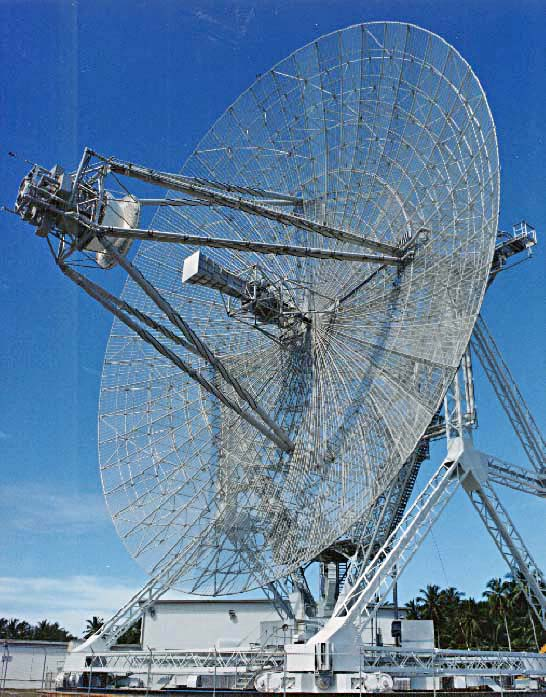
\includegraphics[width=0.9\textwidth]{Fixed_radar_antenna}
\caption{Fixed radar antenna}\label{fig:fixed_radar_antenna}
\end{minipage}\hfill
\begin{minipage}{0.3\textwidth}
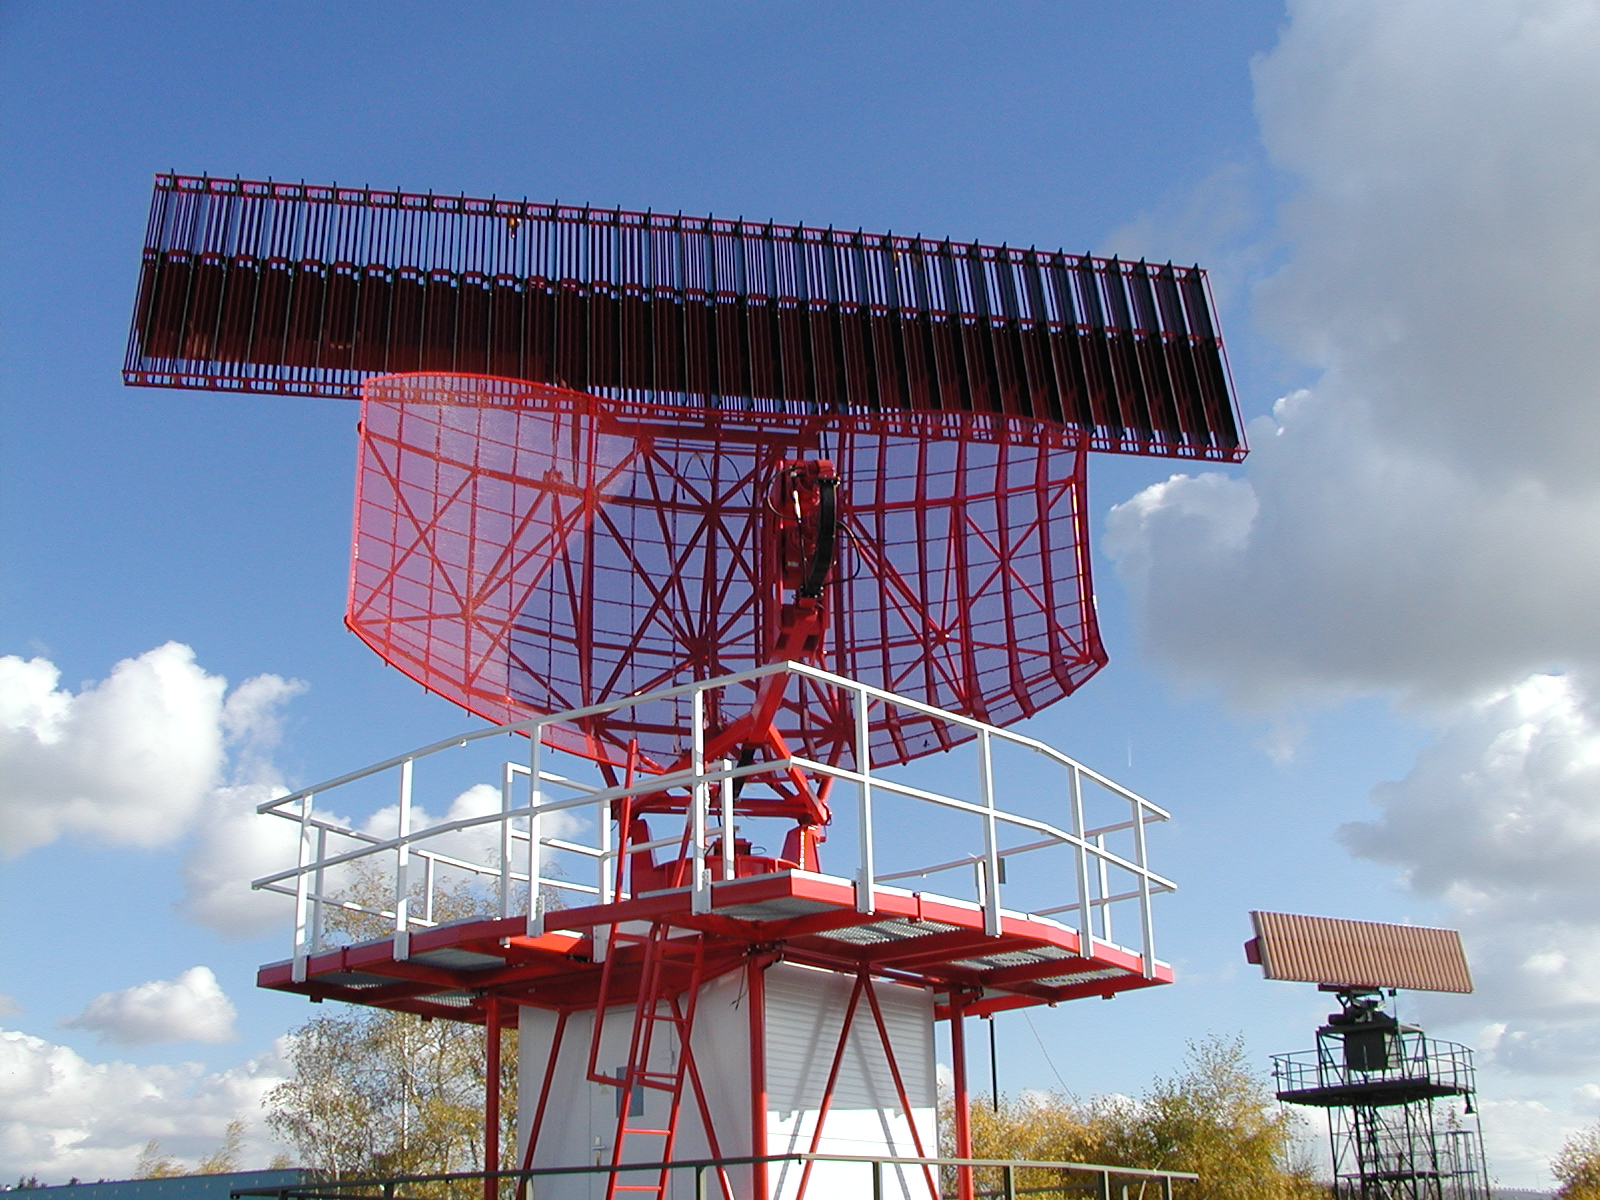
\includegraphics[width=0.9\textwidth]{Rotating_radar_antenna}
\caption{Rotating radar antenna}\label{fig:rotating_radar_antenna}
\end{minipage}\hfill
\begin{minipage}{0.3\textwidth}
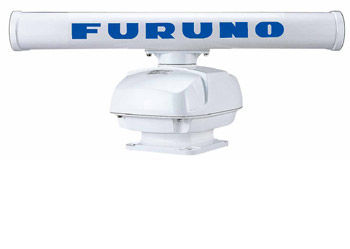
\includegraphics[width=0.9\textwidth]{Maritime_radar_antenna}
\caption{Maritime radar antenna}\label{fig:maritime_radar_antenna}
\end{minipage}
\end{figure}

\subsection{History}
The fist implementation of an instrument that were able to detect the presence of distance metallic objects by radio waves was done by Christian Hülsmeyer in 1904. His invention did not measure the distance to objects, but whether there was an object in the direction of the instrument. The radar as we know it today was introduced in the mid to late 1930's, with world war two triggering a research to improve the still immature technology to be used in military applications. After the war, the technology matured and where put in use in several civil applications, where air traffic control, maritime safety and weather monitoring is the most common.

\subsection{Principles}
The electromagnetic waves that a radar emits travels at the speed of light in air and vacuum. It reflects back when there is a change in the density of the medium it is travelling through, which is what happens when radio waves hit targets. Electrically conductive materials tends to be good reflectors, since they have a very different atomic density than air. On the other hand, materials with poor conductivity, and also some magnetic materials, then to absorb radio waves good. Like light, there is many ways an incoming radio wave can be reflected, primarily dependent on the geometry of the target. A corner with angles less than 180\degsym{} will reflect the incoming radio waves directly back to the sender, and is a good thing on targets that want to be visible on a radar. This principle are the basis for radar reflectors commonly used to boos the radar signature on smaller vessels, see Figure~\ref{fig:corner_reflector}.
\begin{wrapfigure}{R}{0.3\textwidth}
\centering
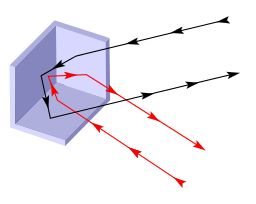
\includegraphics[width=0.25\textwidth]{Corner_reflector}
\caption{Corner reflector}\label{fig:corner_reflector}
\end{wrapfigure}
The opposite is used on targets that try to minimize their radar signature, and is the reason why stealth vessels and aircraft are tiled by flat areas. 
\begin{figure}
\centering
\begin{minipage}{0.3\textwidth}
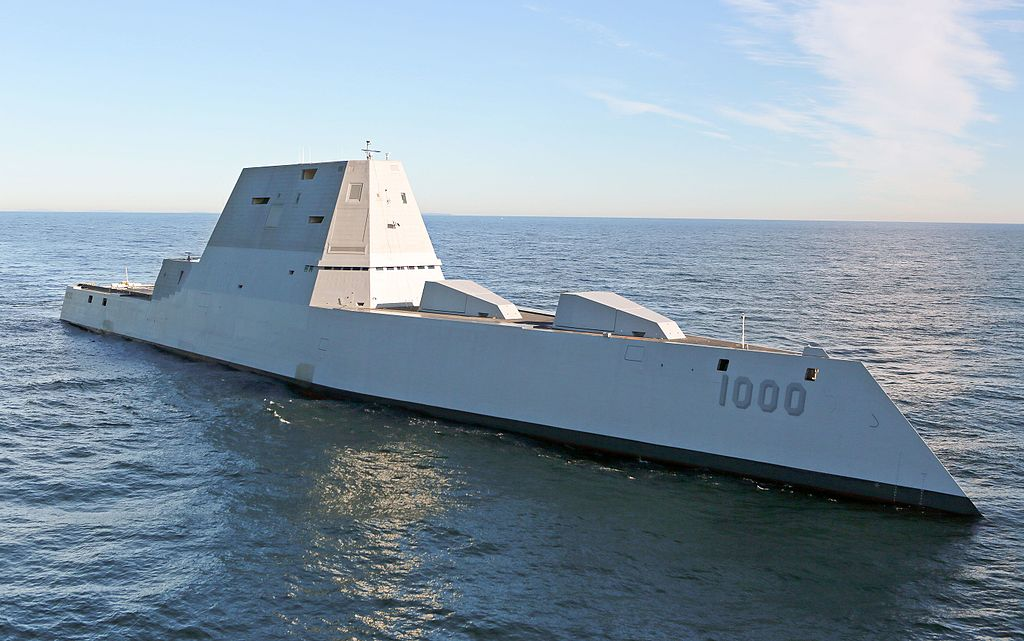
\includegraphics[width=0.9\textwidth]{USS_Zumwalt}
\caption{USS Zumwalt}\label{fig:uss_zumwalt}
\end{minipage}\hfill
\begin{minipage}{0.3\textwidth}
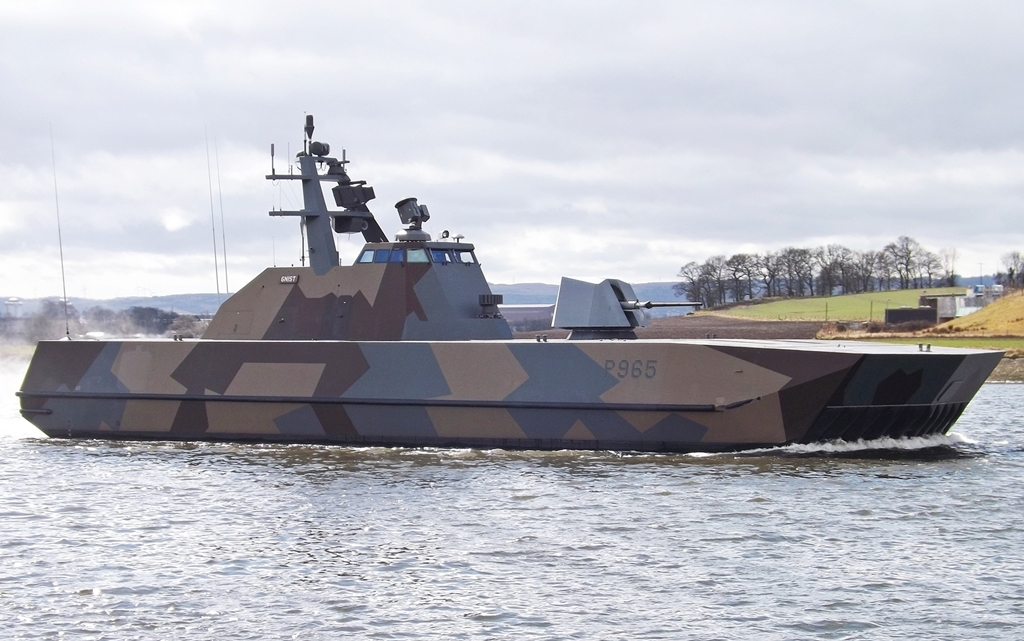
\includegraphics[width=0.9\textwidth]{KNM_Gnist}
\caption{KNM Gnist}\label{fig:knm_gnist}
\end{minipage}\hfill
\begin{minipage}{0.3\textwidth}
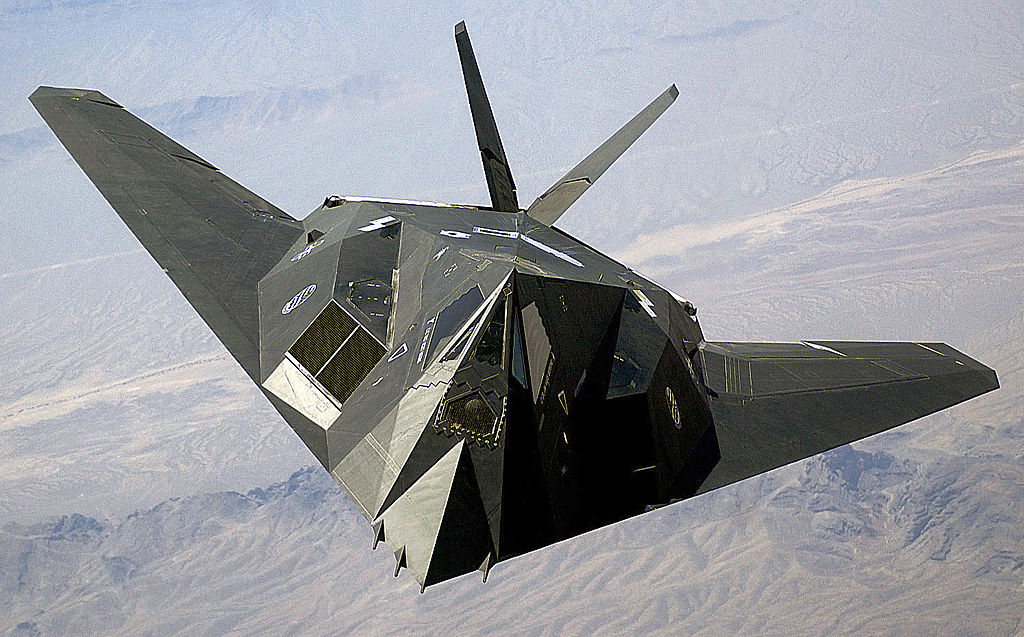
\includegraphics[width=0.9\textwidth]{Figures/F-117_Nighthawk}
\caption{F177 Nighthawk}\label{fig:f177_nighthawk}
\end{minipage}
\end{figure}

\section{AIS}
The \acrfull{ais} is a maritime safety and information system primarily designed for collision avoidance. \gls{ais} works by broadcasting messages on the \gls{vhf} band at irregular intervals with information on the vessels. \gls{ais} transceivers are required on international voyaging vessels over 300 \gls{gross_tonnage}, and on all passenger vessels. \gls{ais} signals are received at bother vessels and shore stations for use in \gls{vts} stations, open tracking databases like \url{www.marinetraffic.com}, fleet-monitoring and search and rescue. Since the \gls{ais} messages contains position, course and speed, \gls{ais} tracks can be overlaid on a map in a chart plotter or on top of a radar image, giving the operator two sensors to verify each other.

\subsection{History}
\gls{ais} was designed and developed by technical comities in the \gls{imo}. Its objective was to enhance vessels safety and efficiency by increasing their ability to see and identify other vessels. The main motivation for adopting \gls{ais} was its independence of humans in operation, since it automatically identifies other vessels and displays the information on the navigational system on the bridge. It also enables automatic calculation of \gls{cpa} and time until \gls{cpa}, in which the navigation system could alarm the bridge on incoming traffic on dangerous course. This gives the navigator on the bridge more and better information for making decisions, but with the caveat that not all vessels have \gls{ais}. In the 2002 \gls{imo} \gls{solas} Agreement, it is required that vessels over 300 \gls{gross_tonnage} and all passenger vessels must be equipped with class A AIS transceivers. A simpler and cheaper \gls{ais} version named class B aimed at smaller vessels and yachts was published in 2006, followed by a large increase in the amount of non-commercial vessels equipped with \gls{ais}.

\subsection{Messages}
\gls{ais} broadcasts both static, dynamic and voyage information with varying intervals based on the vessels speed, status and on request from shore stations. Static, dynamic and voyage messages are listed in Table~\cref{tab:static-ais,tab:dynamic-ais,tab:voyage-ais}. When the \gls{ais} standard was developed, the peak traffic situations in the two most densely trafficked waterways, Singapore and Dover Straits, where used to calculate the update frequency for the AIS system. Based on these two locations and a desire to keep the number of reports per minute below 2000, the dynamic information report intervals for class A and B was set as in Table~\ref{tab:classA_reporting_intervals} and~\ref{tab:classB_reporting_intervals} respectively~\cite{IALA2004}. Static information is transmitted every 6 minutes, and on request from \gls{vts} stations. \gls{ais} transceivers are utilizing two reserved \gls{vhf} channels; AIS 1 --- 87B (161.975MHz) and AIS 2 --- 88B (162.025MHz) to improve robustness against interference. An important note is that \gls{ais} transceivers are alternating which channel they are transmitting on, which means that if a receiver is only listening on one channel, the effective update rate halves.

\begin{table}
	\begin{tabularx}{\textwidth}{XX}
	\toprule
	\multicolumn{2}{c}{Static AIS information} \\
	\midrule
	MMSI & Maritime Mobile Service Identity \\
	Call sign & Maritime radio (VHF) call sign \\
	Name & Name of vessel \\
	IMO Number & Vessel IMO number \\
	Length and beam & \\
	Location of positioning fixing antenna & \\
	Height over keel & \\
	\bottomrule
	\end{tabularx}~\caption{Static AIS information}\label{tab:static-ais}

	\vspace{0.5 cm}

	\begin{tabularx}{\textwidth}{XX}
	\toprule
	\multicolumn{2}{c}{Dynamic AIS information} \\
	\midrule
	Position & In WGS84 frame \\
	Position accuracy & Better or worse that 10 meter \\
	Position time stamp & UTC in whole seconds \\
	Course over ground (COG) & \\
	Speed over ground (SOG) & \\
	Heading & \\
	Navigational status & \\
	Rate of turn (ROT) & \\
	\bottomrule
	\end{tabularx}~\caption{Dynamic AIS information}\label{tab:dynamic-ais}

	\vspace{0.5 cm}

	\begin{tabularx}{\textwidth}{XX}
	\toprule
	\multicolumn{2}{c}{Voyage AIS information} \\
	\midrule
	Draught & Depth in water \\
	Hazardous cargo & Type \\
	Destination & Name of place \\
	Estimated time of arrival (ETA) & \\
	Route plan / waypoints & \\
	Number of persons on board & \\
	\bottomrule
	\end{tabularx}~\caption{Voyage AIS information}\label{tab:voyage-ais}
\end{table}

\begin{table}
	\centering
	\begin{tabularx}{0.8\textwidth}{b s}
	\toprule
	Vessels status & Reporting Interval \\
	\midrule
	Ship at anchor or moored \newline and not moving faster than 3 knots & 3 minutes \\
	Ship at anchor or moored \newline and moving faster than 3 knots & 10 seconds \\
	Ship 0--14 knots & 10 seconds \\
	Ship 0--14 knots and changing course & 3.3 seconds \\
	Ship 14--23 knots & 6 seconds \\
	Ship 14--23 knots and changing course & 2 seconds \\
	Ship > 23 knots & 2 seconds \\
	Ship > 23 knots and changing course & 2 seconds \\
	\bottomrule
	\end{tabularx}~\caption{Class A Reporting Intervals}\label{tab:classA_reporting_intervals}

	\vspace{0.5 cm}

	\begin{tabularx}{0.8\textwidth}{b s}
	\toprule
	Vessels status & Reporting Interval \\
	\midrule
	Ship < 2 knots & 3 minutes \\
	Ship 2--14 knots & 30 seconds \\
	Ship 14--23 knots & 15 seconds \\
	Ship > 23 knots & 5 seconds \\
	Search and Rescue aircraft & 10 seconds \\
	Aids to navigation & 3 minutes \\
	AIS base station & 10 seconds \\
	\bottomrule
	\end{tabularx}~\caption{Class B Reporting Intervals}\label{tab:classB_reporting_intervals}

\end{table}

\subsection{Class A}
Class A \gls{ais} transceivers are designed for \gls{sotdma} transmission, which is a way of reserving transmission time slot for the next broadcast. \gls{sotdma} is based on \gls{tdma}, with an extension allowing for self organizing of time slots compared to \glspl{tdma} dedicated timing manager. This effectively gives class A AIS transmissions priority over Class B equipment which may not have \gls{sotdma}. Class A transceivers are also required to have build-in display, minimum transmission power of 12.5W, ability to filter targets and communication interfaces like \gls{rs232} and \gls{nmea}.

\subsection{Class B}
Class B \gls{ais} transceivers are designed to be simpler and cheaper than Class A transceivers, which is accomplished through less strict requirements for hardware and operation. Class B \gls{ais} transmits at lower power, usually 2W and transmits at larger time intervals than Class A, see Table~\ref{tab:classB_reporting_intervals}. It is not required to have a build-in display and can use both \gls{cstdma} and \gls{sotdma} for transmission. \gls{cstdma} is a simpler approach to time division than \gls{sotdma} since it only listen for a single time slot to be unused before it transmits.

\section{Tracking}
\subsection{Overview}
Tracking, in this context, is the process of estimating the state of stationary and moving targets that are observed by a system without included association data. The challenge is to know which measurements belong together over time, often refereed to as the data association problem. An observation system can be a radar, sonar or any other sensor that, passively or actively, detects objects within an area or volume. Any observation system will be prone to noise, both in form of internal- and external noise from the environment. This noise will cause false measurements that the tracking system must take care of. These false measurements are often referred to as clutter.

In this work `tracking algorithm' will be used to describe the main logic in a tracking method or approach, while `tracking system' will be used on complete systems with everything around the main algorithm included. A tracking system can be defined as: \emph{A system that process consecutive measurements from one or more observation system and associates measurement from the same target into tracks with initialization of new tracks and termination of dead tracks}. A track is a sequence of states associated with a subset of all measurements from the observation systems. 

Tracking is a relative new filed of study, driven by the military and aerospace industry and enabled by the development of microprocessors and computers from the 1960's. The applications ranges from sonar tracking on both submarines and navy vessels, to air control and missile guidance. This historical background is likely the reason for most published papers using these types of applications as background for testing. In recent years, tracking people and vehicles from visual- and \gls{sar} imagery have also become a topic in the research community~\cite{Carthel2007,Carthel2007a,Coraluppi2000}. New applications areas like oceanography, autonomous vehicles and biomedical research have also found use of tracking~\cite{Wolf2010,Svec2014,Vo2015}.

There are several factors contributing to the challenge of good tracking; \gls{clutter}, lower than unity \gls{Pd}, multiple detections of the same vessel and wakes. \Gls{clutter} is a term for unwanted measurements or noise, which is inherent in every observation system. For a maritime radar, this can be caused by waves, rain, snow, birds or shore echo. A common assumption on clutter is to assume the amount being Poisson distributed, and spatially uniformly distributed. \gls{Pd} is a measure of how persistent the target is in the measurements, and will vary much between different types of targets, primarily dependent on their size, construction material and shape. Multiple detections of each target can occur when the target is large and have several distinct areas which reflects radar waves better than the rest of the vessel, for instance when the hull of a boat is made from fibreglass and the metal objects inside is reflecting. Wakes are reflection caused by the turbulent water behind a moving object, which can be a problem for both sonar and maritime- and air-radar.

\subsection{Single-target tracking}
The simplest approach to tracking is single-target tracking, where it is assumed that there are only one target in the measurement area, and any other measurement is regarded as either extra measurements of the target or \gls{clutter}. 

\subsubsection*{\gls{nnf}}
The simplest single-target tracking algorithm is the \gls{nnf}, where the closest measurement is always selected~\cite{Bar-Shalom1998}. This approach is very vulnerable to clutter and dense multitarget scenarios, which is probably the reason its usage is very sparse. 

\subsubsection*{\gls{pdaf}}
The arguably best single-target tracking algorithm is \gls{pdaf}, which calculates probabilities of all target to measurement association for all measurement inside its gate. A gate is an ellipse (2D) or ellipsoid (3D) which outlines the confidence area / volume for a predicted state and covariance for a given confidence value. The state update is then based on a weighted sum of measurement innovations where the weightings are the probabilities for their respective innovations. One of the main assumptions in \gls{pdaf} is that all the measurements inside its gate contains information about the targets true state. This assumption performs well in single-target scenarios since targets often create more than measurements, and thus using all measurements in state estimation effectively rejects much of the \gls{clutter} in each \gls{scan}.

\subsection{Multitarget tracking}
A more generalized approach assuming that there can be any number of targets is called multitarget tracking. The problem expands to jointly estimate both the number of targets and their trajectories since targets can enter and leave the surveillance area. 

While a large number of tracking techniques have been developed, the three most used are \gls{jpdaf}, \gls{mht} and \gls{rfs}~\cite{Vo2015}. Compared to \gls{mht} and \gls{jpdaf}, \gls{rfs} is a relatively new approach to tracking, and is not  matured the same way \gls{mht} and \gls{jpdaf} are. \gls{mht} and \gls{jpdaf} also differs from \gls{rfs} in that they both do data association and filtering, whereas \gls{rfs} directly seeks both optimal and suboptimal estimates of the multitarget state~\cite{Vo2015}.

\subsubsection{JPDAF}
\gls{jpdaf} is a multitarget expansion of \gls{pdaf} which is a single-target tracking technique. PDAF calculates joint posteriori association probabilities for every target in every scan. Each targets probability is a weighted sum of probabilities, where the weights are the key difference between \gls{pdaf} and \gls{jpdaf}. Like \gls{mht}, \gls{jpdaf} suffers from high computational cost, and an efficient implementation approach exist and is patented by QinetiQ~\cite{Horridge}.

\subsubsection{MHT}
\gls{mht} is a decision logic which generates and maintains alternative hypotheses when new \glspl{measurement} are received and within the gate. By making several possible hypotheses, the decision on which \gls{measurement} to choose can be propagated into the future when more information is available. MHT is multi frame method, meaning it has the ability to utilize multiple scans to make better decisions. Each hypothesis is given a \gls{score} based on a likelihood ratio as a reflection of how well the measurement fits the model, which are accumulated to evaluate the combinations of consecutive \glspl{measurement}.

In contrast to the \gls{pdaf} and \gls{jpdaf} methods who suffers from track \gls{coalescence}, \gls{mht} methods split when in doubt. The idea of using multiple hypotheses was first introduced by~\cite{Singer1974}, but the first complete algorithm was presented in~\cite{Reid1979}, where a \gls{homht} was developed. Following this, a \gls{tomht} was proposed in~\cite{Kurien1990} and the \gls{score} function for \gls{mht} was later deduced and discussed in~\cite{Bar-Shalom2007} since no explicit track-score function were given in~\cite{Kurien1990}. \gls{mht} is, in the same way as \gls{pdaf}/\gls{jpdaf}, developed under two main assumptions; that at most one \gls{measurement} can originate from each \gls{target} in each scan, and that a \gls{target} does not necessarily show on every scan, or in other words, \gls{Pd} less than 1. The \gls{mht} approach to tracking and data association was for a long time dismissed by many because of its computationally large cost. The dramatic increase in computational capability from the 1980's to the late 2010's have, however, lead to a new spring for \gls{mht}, with an increasing interest for use in tracking system. In 2004 Blackman stated that \say{Multiple hypothesis tracking is generally accepted as the preferred method for solving the data association problem in modern multiple \gls{target} tracking system}~\cite{Blackman2004}. Already in 2001 did Blackman publish a demonstration that \gls{mht} is capable of real-time demands~\cite{Blackman2001}.

\gls{mht} comes in two variations, \gls{homht} and \gls{tomht}. They differ in their approach to arrange the measurements into hypotheses in that \gls{homht} builds hypotheses that are different ways of organizing the measurements into tracks, while \gls{tomht} maintains already existing tracks and a hypothesis is only a possible track for a single target and not all targets. This means that in \gls{tomht}, to select the 


\subsubsection{\gls{rfs}}
\Gls{rfs} is a family of Bayesian methods and filters that is based on representing a multitarget state as a finite set of single target states. By not having the multitarget states represented as a vector, the estimation error is more meaningful and mathematically consistent. This is because the vector representation is ordered, and thus the only meaningful way of representing the estimation error would be to minimize the estimation error over all permutations of states. This can be represented as distances between finite sets, and is a much more well defined and understood concept. 
% \Gls{rfs} method are, like \gls{pdaf} and \gls{jpdaf}, based on representing the history of a target as a prior probability density.

The \gls{rfs} approach to multi sensor multitarget tracking was done by Mahler in 1994, which lay the foundation for the development of \gls{fisst}. One popular filter based on \gls{rfs} is the \gls{phd} filter. The \gls{phd} filter is an approximation of the multitarget Bayes filter derived by Mahler using \gls{fisst}~\cite{Vo2015}. The \gls{phd} filter estimates the number of targets and then selects the same numbers highest probable tracks. One large drawback with the \gls{phd} filter is its assumption that the predicted multitarget \gls{rfs} is Poisson distributed. This assumption is relaxed in the \gls{cphd} filter where the prior and predicted multitarget densities are independently and identically distributed clusters. \clearpage 
	%!TEX root = ../TTK4900-MHT.tex

\chapter{Implementation}\label{chapter:implementation}
Implementation here. \clearpage 
	%!TEX root = ../TTK4900-MHT.tex

\chapter{Results}\label{chapter:results}
\section{Testing scheme}
The performance evaluation of the MHT tracking system is tedious in that it is necessary to test very many different situations to get a good understanding of how the system is performing. The two largest factors contributing to the difficulty is the random nature of the clutter and lost detections. It is also desirable to evaluate the initialization and tracking performance under both varying environmental (external) conditions and tuning (internal) setting. We want good tracking of targets with low probability of detections in cluttered environment, and secondly it must be able to do this within the time frame of the radar rotation period. The initialization module must be able to detect targets with probability of detection lower than unity without initializing too may false tracks into the MHT algorithm. The testing is separated into two parts; initialization and tracking.

The performance metrics for the initialization module is how long time it takes to initialize the correct tracks, which is tested under a range of internal and external conditions, see (\ref{eq:init_test_table}). All combinations of these parameters were simulated on all scenarios, see Table~\ref{tab:ais_scenarios}, which are the same routes but with different \gls{ais} configurations. From these simulations, the time to initiate true targets and amount of false targets are calculated. A track is categorized as correct initialized if the state difference between the true track and the initial track is less that a threshold. All initial tracks that does not correspond to a true track is categorized as erroneous. To analyse the impact of the erroneous tracks, the lifespan of falsely initiated tracks is plotted to see whether they die out at the same rate as they are initiated, or if they accumulate.  
\begin{equation}\label{eq:init_test_table}
\begin{split}
\V{P_D} &= \begin{bmatrix} 1.0 & 0.8 & 0.6 \end{bmatrix} \\
\V{M/N} &= \begin{bmatrix} 	(1/1) & (1/2) & (1/3) & (1/4) \\
							(2/2) & (2/3) & (2/4) & (2/5) \\
							(3/3) & (3/4) & (3/5) & (3/6)
		   \end{bmatrix} \\
\V{\lambda_\phi} &= \begin{bmatrix} 0 & 2\cdot10^{-6} & 4\cdot10^{-6} \end{bmatrix}
\end{split}
\end{equation}

When testing the tracking performance, it is desirable to remove the variable of initialization to better see difference in \emph{tacking} rather than \emph{initialization}. Therefore are all the simulations testing tracking performance carried out with all targets correctly initialized at initial time, and with the initiator set to \(M=2, N=4\) such that the unused measurements from the tracking algorithm would be treated as normal. This would also give lost targets a change to get re-initialized, which is an important property for any safety critical system.
\begin{equation}\label{eq:tracking_test_table}
\begin{split}
\V{P_D} &= \begin{bmatrix} 1.0 & 0.8 & 0.6 \end{bmatrix} \\
\V{N} &= \begin{bmatrix} 1 & 3 & 6 & 9 \end{bmatrix} \\
\V{\lambda_\phi} &= \begin{bmatrix} 0 & 2\cdot10^{-6} & 4\cdot10^{-6} \end{bmatrix}
\end{split}
\end{equation}
Since the targets are initialized perfectly in every situation, we are interested in how good our system is able to \emph{keep} on the tracks. We measure this by means of the Euclidean distance between the estimated and true track (\ref{eq:euclidian_distance_vector}).
\begin{equation}
	\Delta P = \| \V{p}_{track}-\V{p}_{target} \|_2
\label{eq:euclidian_distance_vector}
\end{equation}
The track is considered correct if \(\Delta P \leq \varepsilon_p\) for all t after initial convergence. If a track is deviating more than the threshold and never return within the threshold again, it is considered lost at the time-step when it exceeded the threshold. If the track should converge after exceeding the threshold, it is considered restored at the time-step it is returning within the limit. The second metric is how close the estimated track is to the true track on average. This is measured in \gls{rms} error of the entire track.

\section{Scenario}\label{sec:scenario}
All simulations in this work is based on a generated scenario, as shown in Figure~\ref{fig:test_scenario}, with black dots marking the initial time and position. The radar range is 5500 meter (~3 \glspl{nm_acr}), which gives an area of surveillance of approximately 95 square km. The scenario contains 16 targets, which all starts inside the observable area of the radar. The scenario contains a mixture of fast and slow moving vessels, some with sharp turns and some almost at stand still. Table~\ref{tab:init_states} shows the initial states of all targets, and the true path is generated once from these initial values.
\begin{figure}[H]
\centering
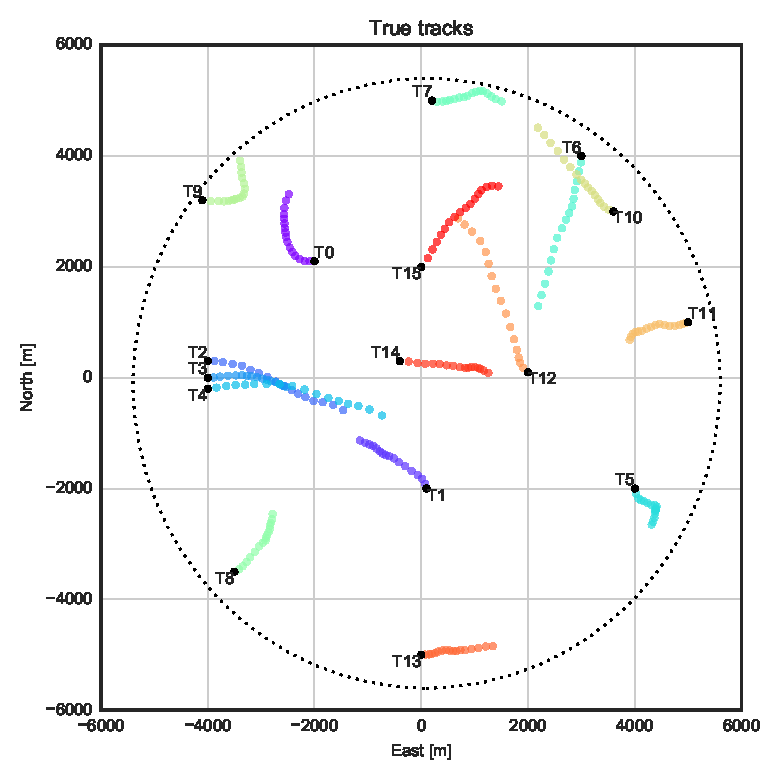
\includegraphics[width = .9\textwidth]{Figures/plots/ScenarioTruth.pdf}
\caption{True tracks}\label{fig:test_scenario}
\end{figure}

\begin{table}[H]
\centering
\begin{tabular}{c c c c c}
\bfseries Target & \bfseries North & \bfseries East & \bfseries North speed & \bfseries East speed \\ 
\toprule
\csvreader[head to column names,respect percent=true]{{Figures/plots/Scenario_Initial_State.csv}}{}
{\T{} & \NP{} & \EP{} & \NS{} & \ES{} \\}
\end{tabular}
\caption{Initial states}\label{tab:init_states}
\end{table}

From this base scenario, five scenarios where generated with different AIS configuration on the vessels, see Table~\ref{tab:ais_scenarios}. The first scenario represent the baseline with only radar information available, whereas the rest have some level of AIS information. Scenario 2 adds three class B AIS transmitters, and is representing a situation where all the targets are smaller vessels with some voluntarily installed AIS transceivers. In scenario 3, all vessels have AIS class B installed. This scenario represents a best case situation regarding yacht and leisure vessels from an autonomous anti collision perspective and is only realistic if AIS class B where to be mandatory for these vessel classes. Scenario 4 is the same as scenario 2, with the difference that the vessels have class A transmitters in stead of class B. This gives them higher and smarter rate of transmission, which in theory should improve tracking under challenging conditions. This scenario can be viewed as a few commercial vessels travelling in between a large group of yachts. The last scenario, where all targets are equipped with class A transmitters is the ultimate situation for any fusion tracking system. This case would be realistic in a crowded professional working area, for instance harbours, fishing areas and off-shore installations. 
\begin{table}
\centering
	\begin{tabularx}{0.5\textwidth}{XXXXXX}
	  \multicolumn{5}{c}{AIS scenario configuration} \\
	  \toprule
	  		 & \multicolumn{5}{c}{Scenario} \\
	  Target & 0 	& 1 	&  2 	&  3	& 4  	\\
	  \midrule
	  0 	& --- 	& --- 	& B 	& --- 	& A 	\\
	  1 	& --- 	& --- 	& B 	& --- 	& A 	\\
	  2 	& --- 	& --- 	& B 	& --- 	& A 	\\
	  3 	& ---	& B 	& B 	& A 	& A 	\\
	  4 	& --- 	& --- 	& B 	& --- 	& A 	\\
	  5 	& --- 	& --- 	& B 	& --- 	& A 	\\
	  6 	& --- 	& --- 	& B 	& --- 	& A 	\\
	  7 	& --- 	& --- 	& B 	& --- 	& A 	\\
	  8 	& --- 	& --- 	& B 	& --- 	& A 	\\
	  9 	& --- 	& --- 	& B 	& --- 	& A 	\\
	  10 	& --- 	& --- 	& B 	& --- 	& A 	\\
	  11	& ---	& B 	& B 	& A 	& A 	\\
	  12 	& --- 	& --- 	& B 	& --- 	& A 	\\
	  13 	& --- 	& --- 	& B 	& --- 	& A 	\\
	  14 	& ---	& B 	& B 	& A 	& A 	\\
	  15 	& --- 	& --- 	& B 	& --- 	& A 	\\
	  \bottomrule
	\end{tabularx}~\caption{AIS scenario configuration}\label{tab:ais_scenarios}
\end{table}

\section{Simulation}
Both initialization- and tracking performance is averaged over a set of 50 Monte Carlo simulations with differently seeded clutter- and detections points. All simulations are done with a sampling interval at 2.5 seconds (24 \gls{rpm}), which is the most common rotation speed on a coastal maritime radar. Each of the 108 initialization variations and 180 track performance simulations where run 50 times with different seeded clutter and misdetections on a dual Intel i7--6700 processor and \gls{ssd} storage. 
 \clearpage 
	%!TEX root = ../TTK4900-MHT.tex

\chapter{Discussion and conclusion}
\label{ch:discussion_conclusion}
 \clearpage  
	% %!TEX root = ../TTK4900-MHT.tex

\begin{appendices}
	%!TEX root = ../TTK4900-MHT.tex

\chapter{Initialization time plot}

\begin{figure}[H]
\centering
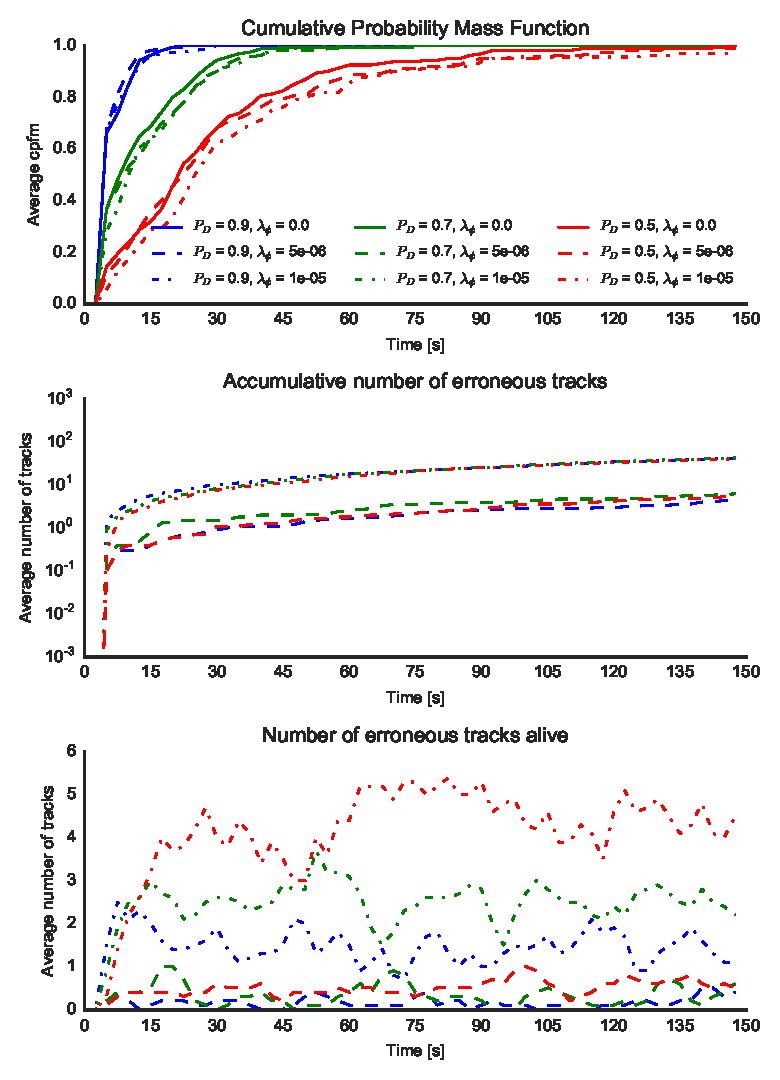
\includegraphics[height = .9\textheight]{Figures/plots/Scenario1_Init-Time(1-1).pdf}
\caption{Initialization time (1/1)}\label{fig:init_time_1-1}
\end{figure}

\begin{figure}
\centering
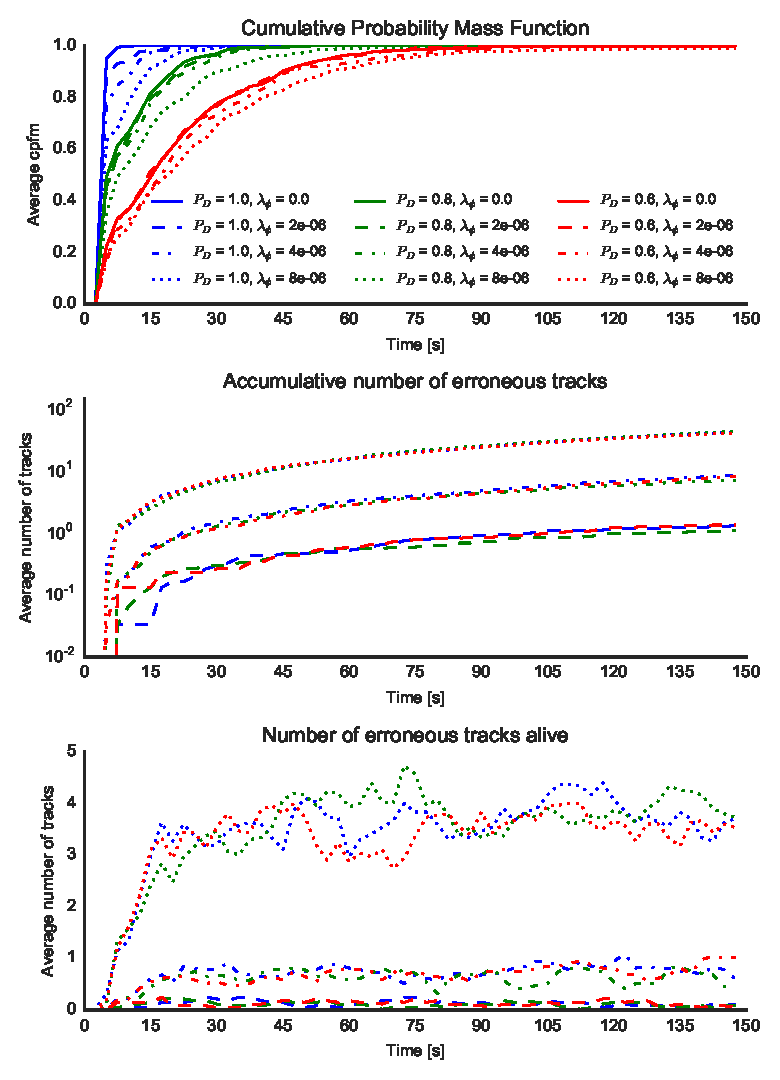
\includegraphics[height = .9\textheight]{Figures/plots/Scenario1_Init-Time(1-2).pdf}
\caption{Initialization time (1/2)}\label{fig:init_time_1-2}
\end{figure}

\begin{figure}
\centering
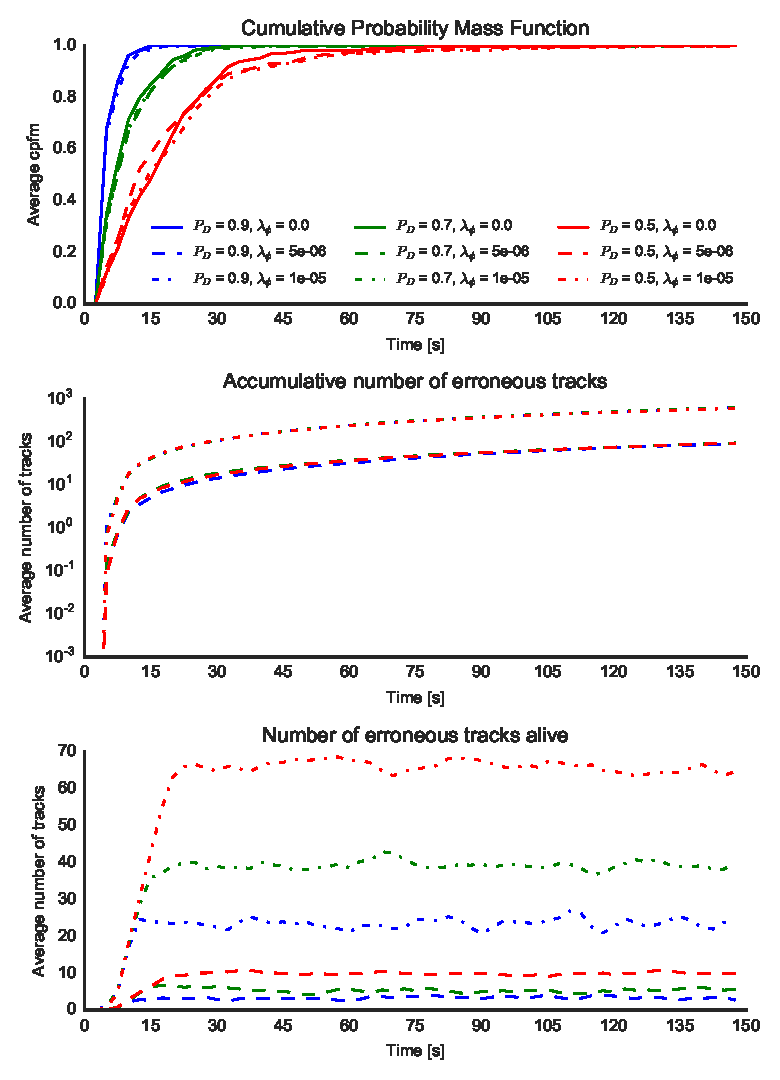
\includegraphics[height = .9\textheight]{Figures/plots/Scenario1_Init-Time(1-3).pdf}
\caption{Initialization time (1/3)}\label{fig:init_time_1-3}
\end{figure}

\begin{figure}
\centering
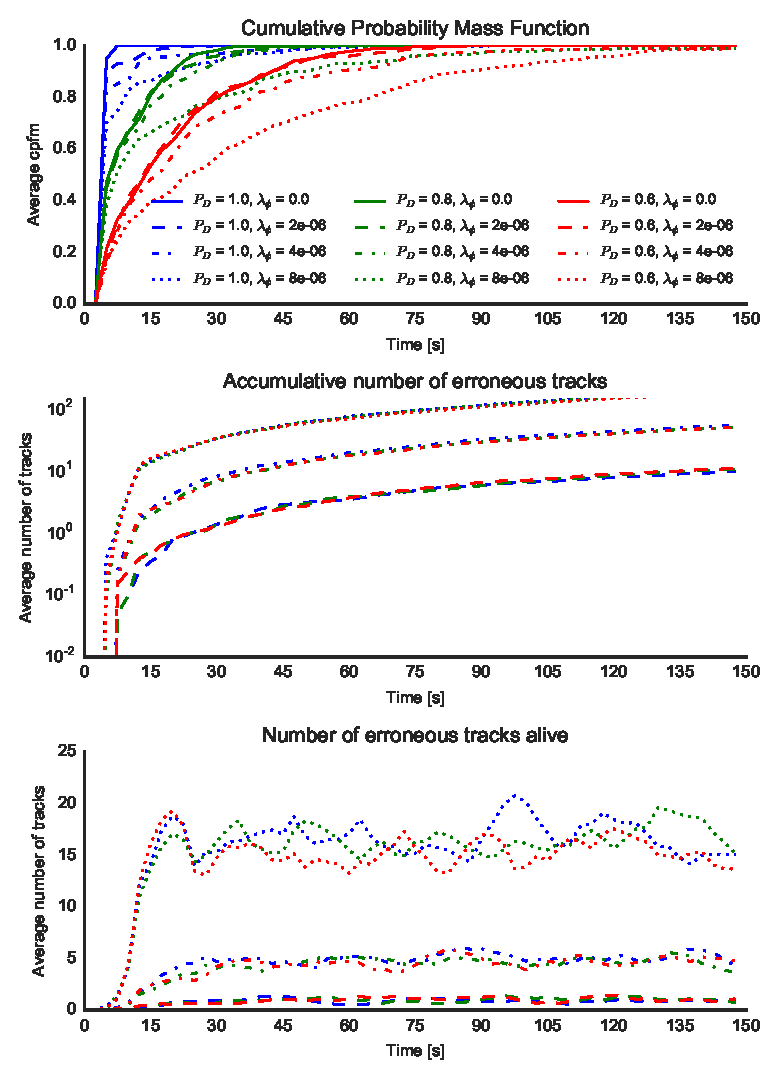
\includegraphics[height = .9\textheight]{Figures/plots/Scenario1_Init-Time(1-4).pdf}
\caption{Initialization time (1/4)}\label{fig:init_time_1-4}
\end{figure}

\begin{figure}
\centering
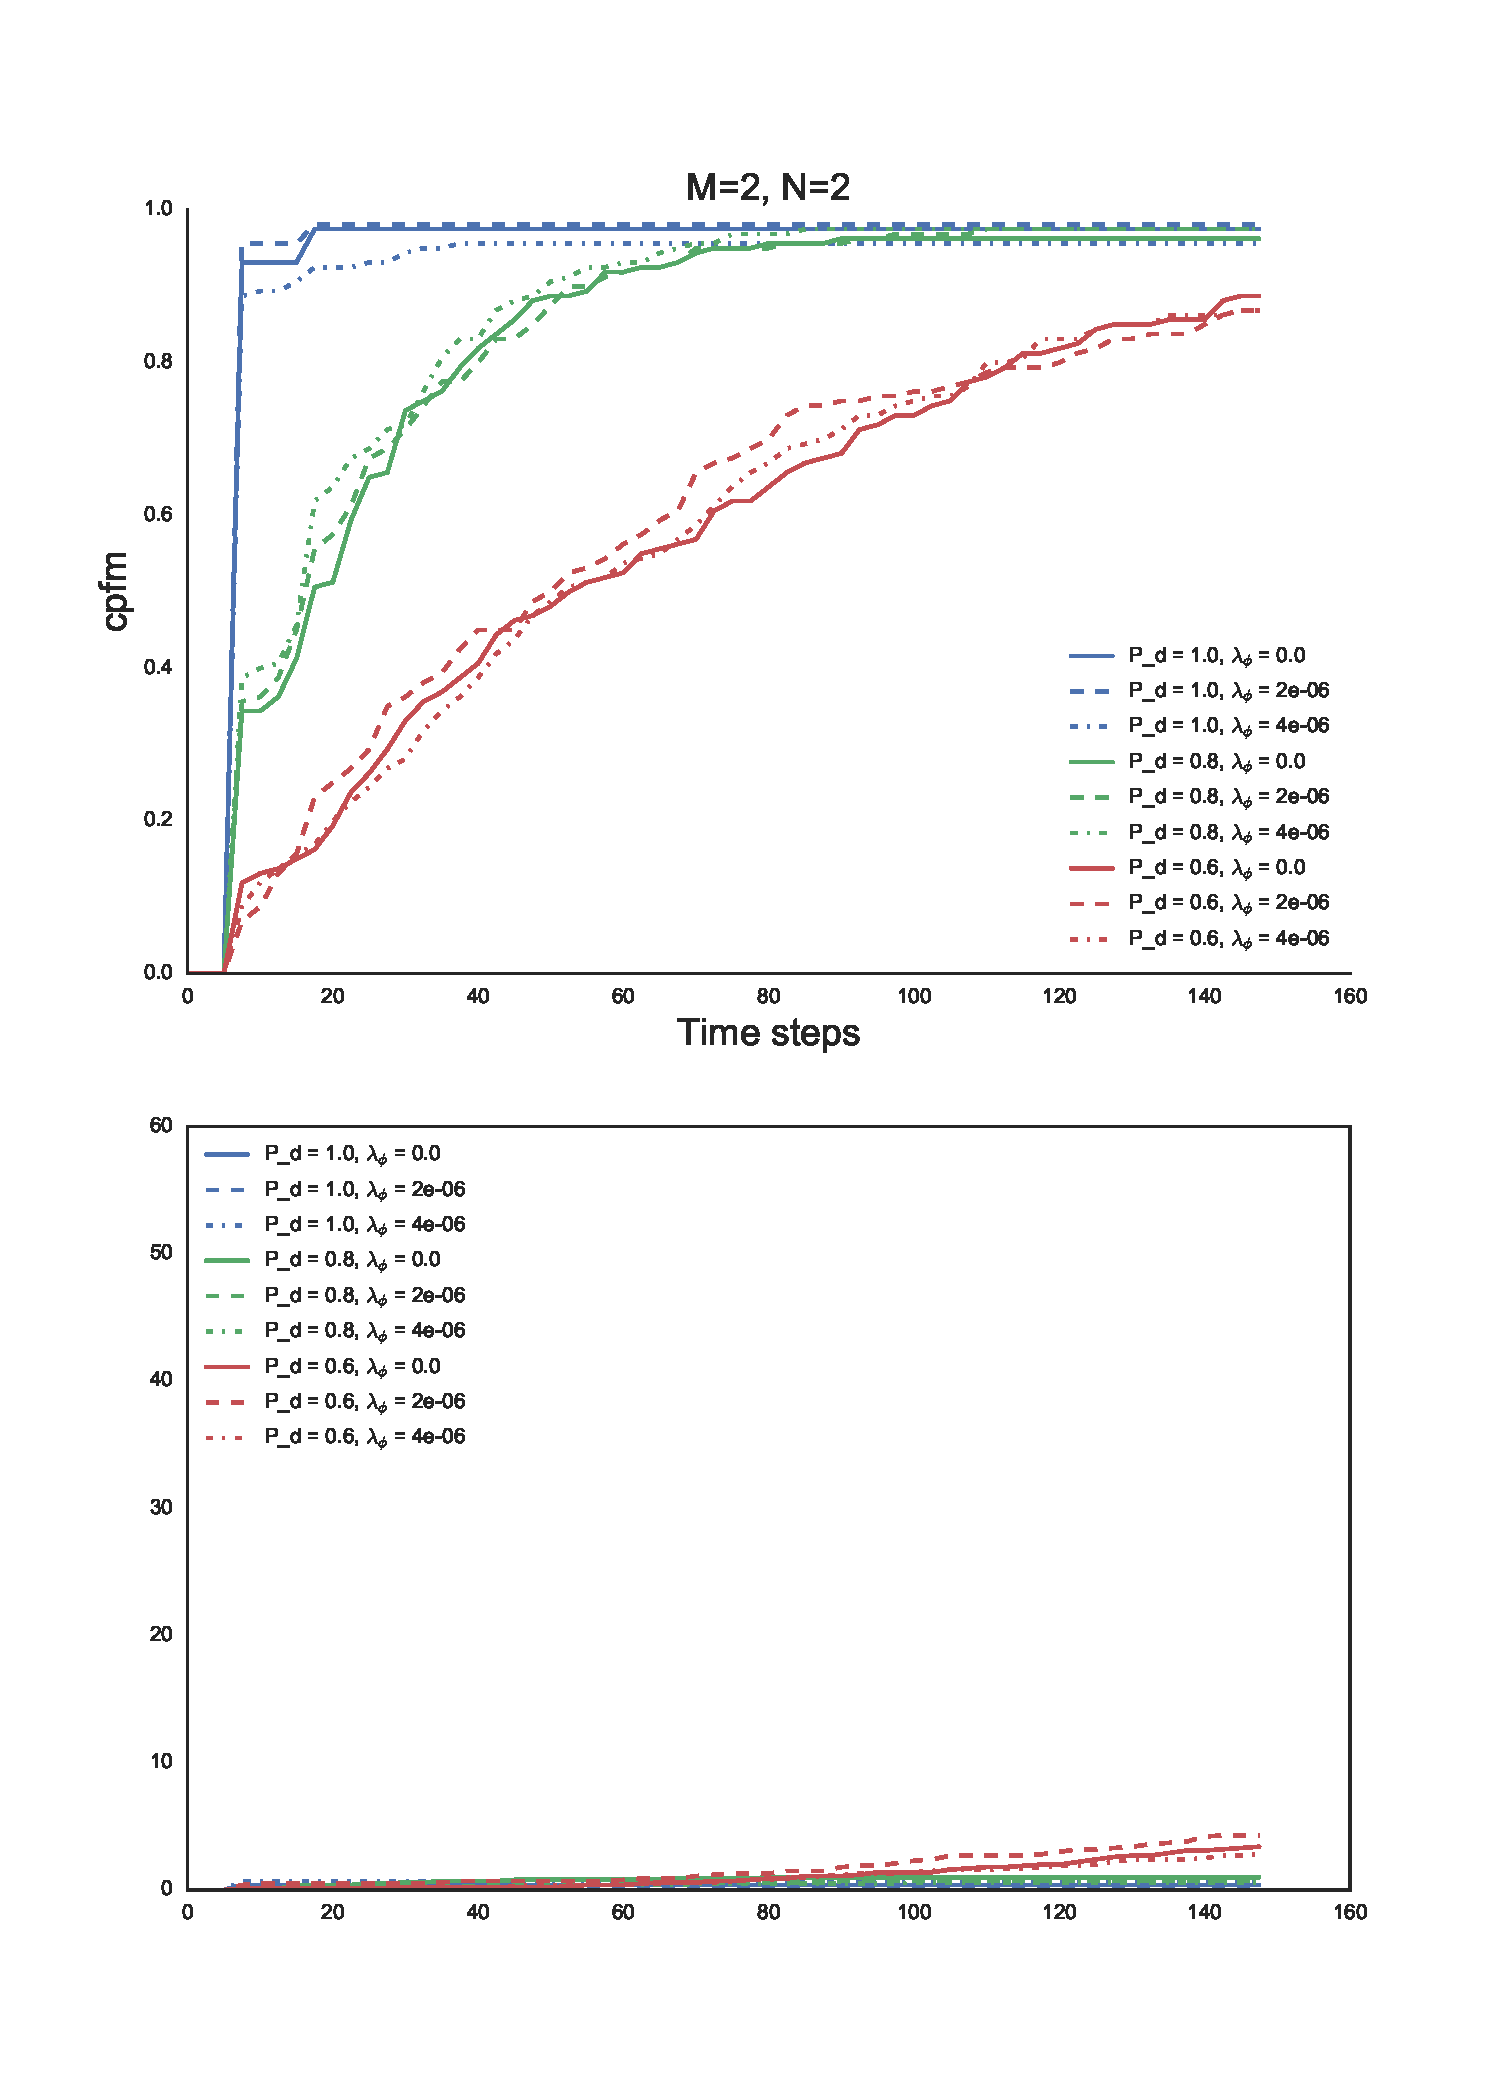
\includegraphics[height = .9\textheight]{Figures/plots/Scenario1_Init-Time(2-2).pdf}
\caption{Initialization time (2/2)}\label{fig:init_time_2-2}
\end{figure}

\begin{figure}
\centering
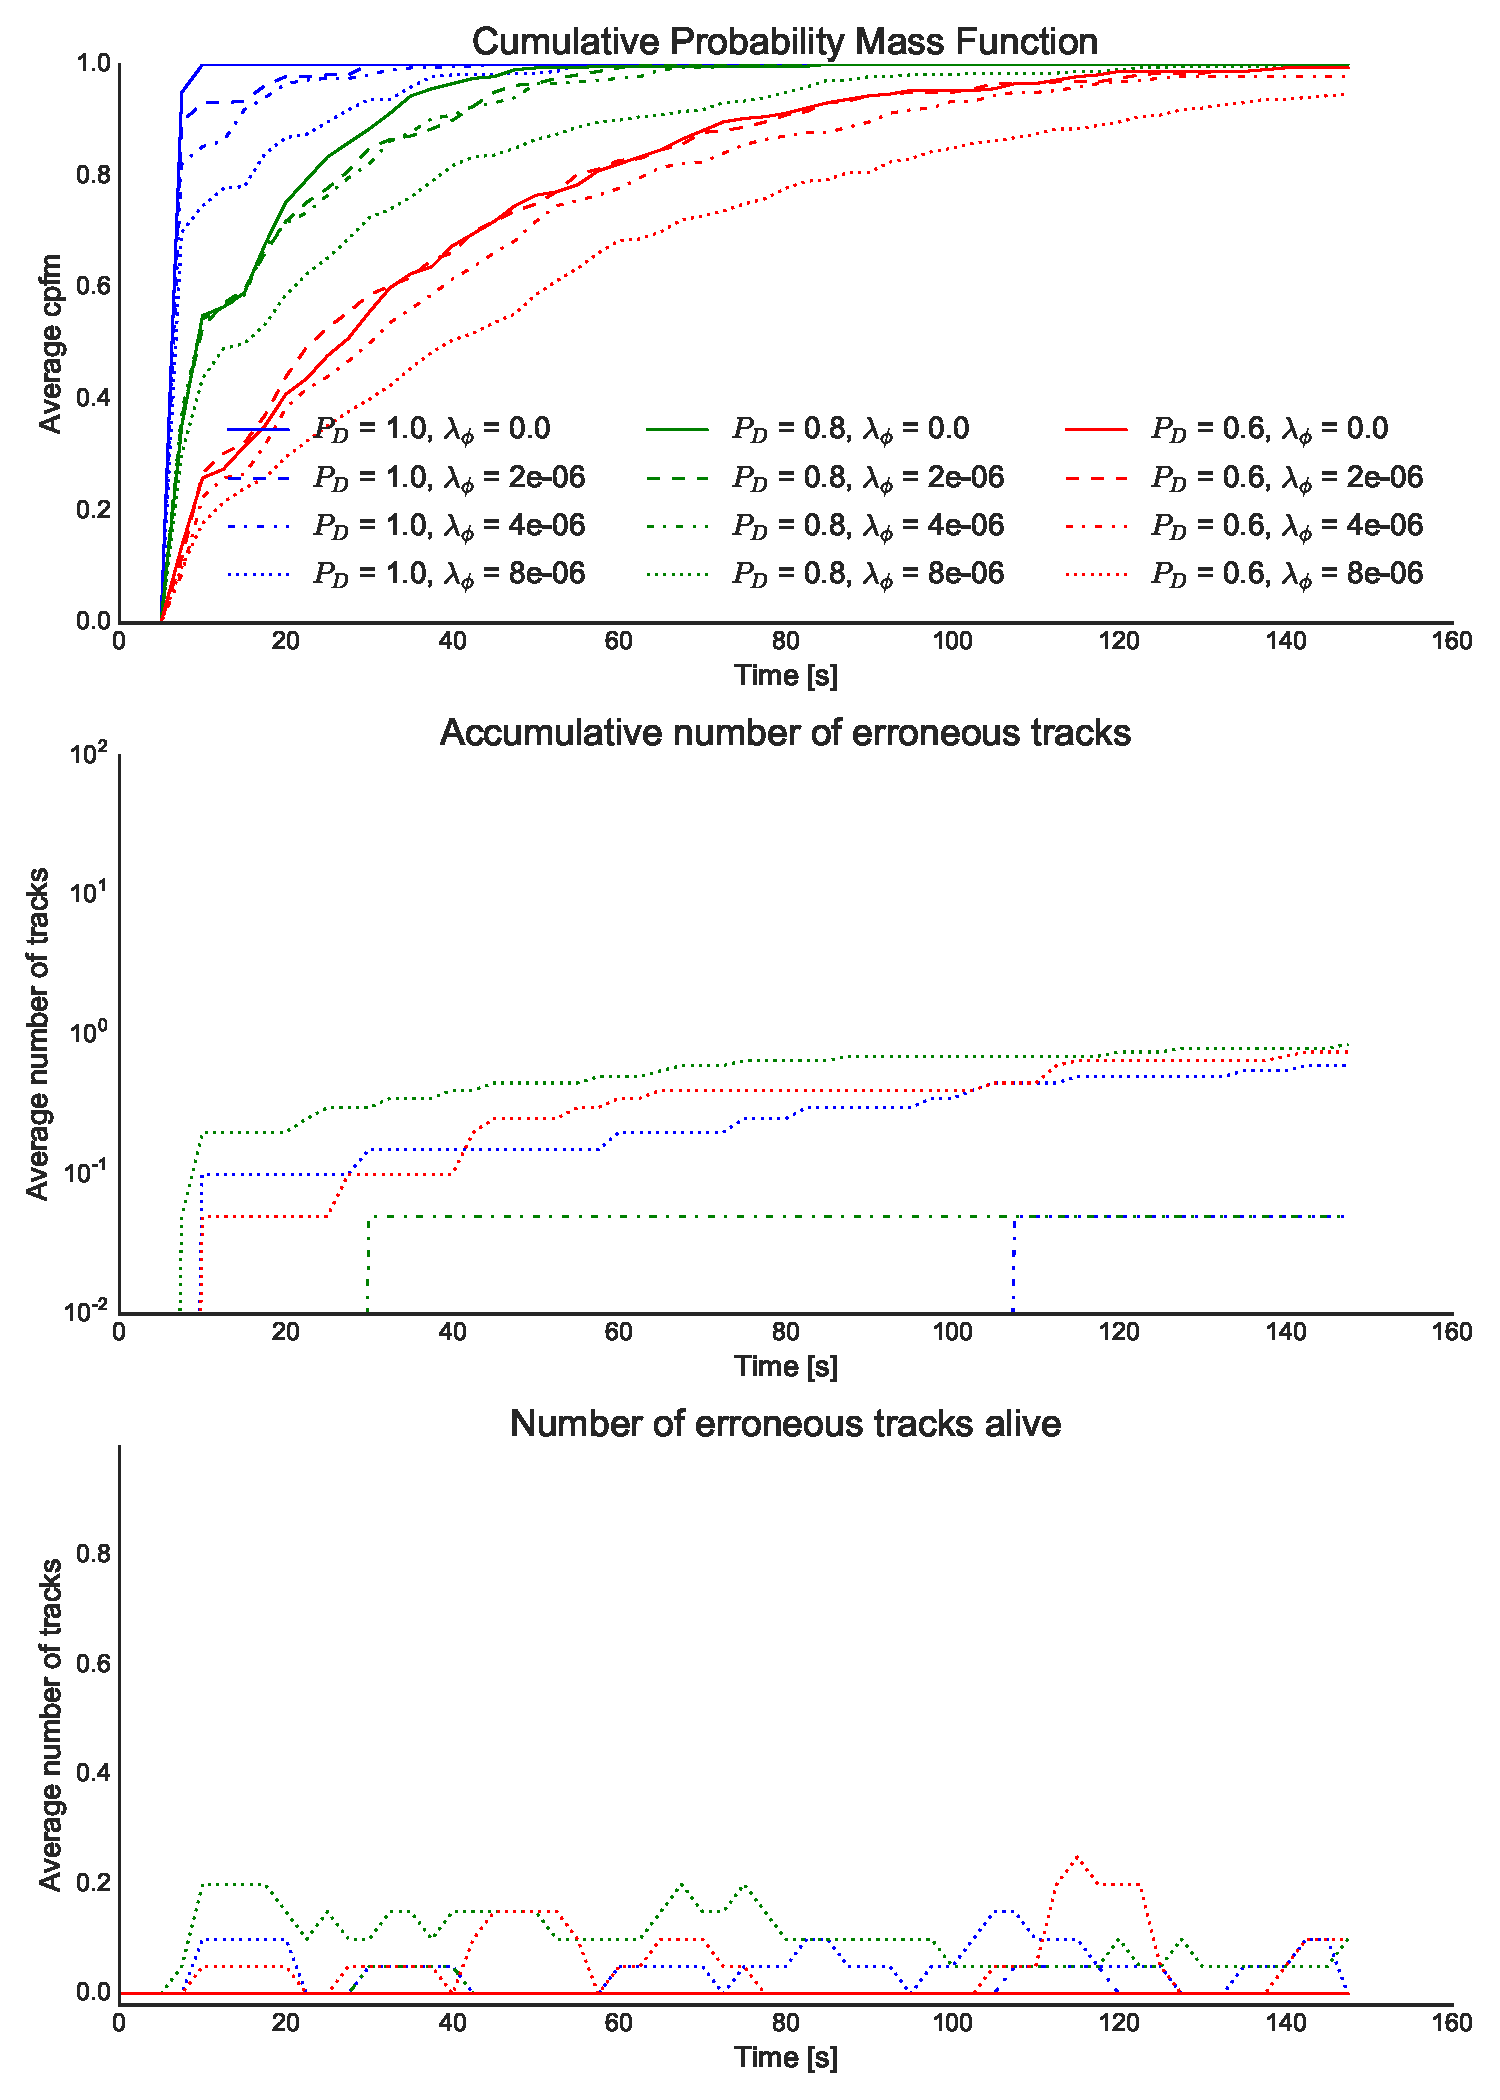
\includegraphics[height = .9\textheight]{Figures/plots/Scenario1_Init-Time(2-3).pdf}
\caption{Initialization time (2/3)}\label{fig:init_time_2-3}
\end{figure}

\begin{figure}
\centering
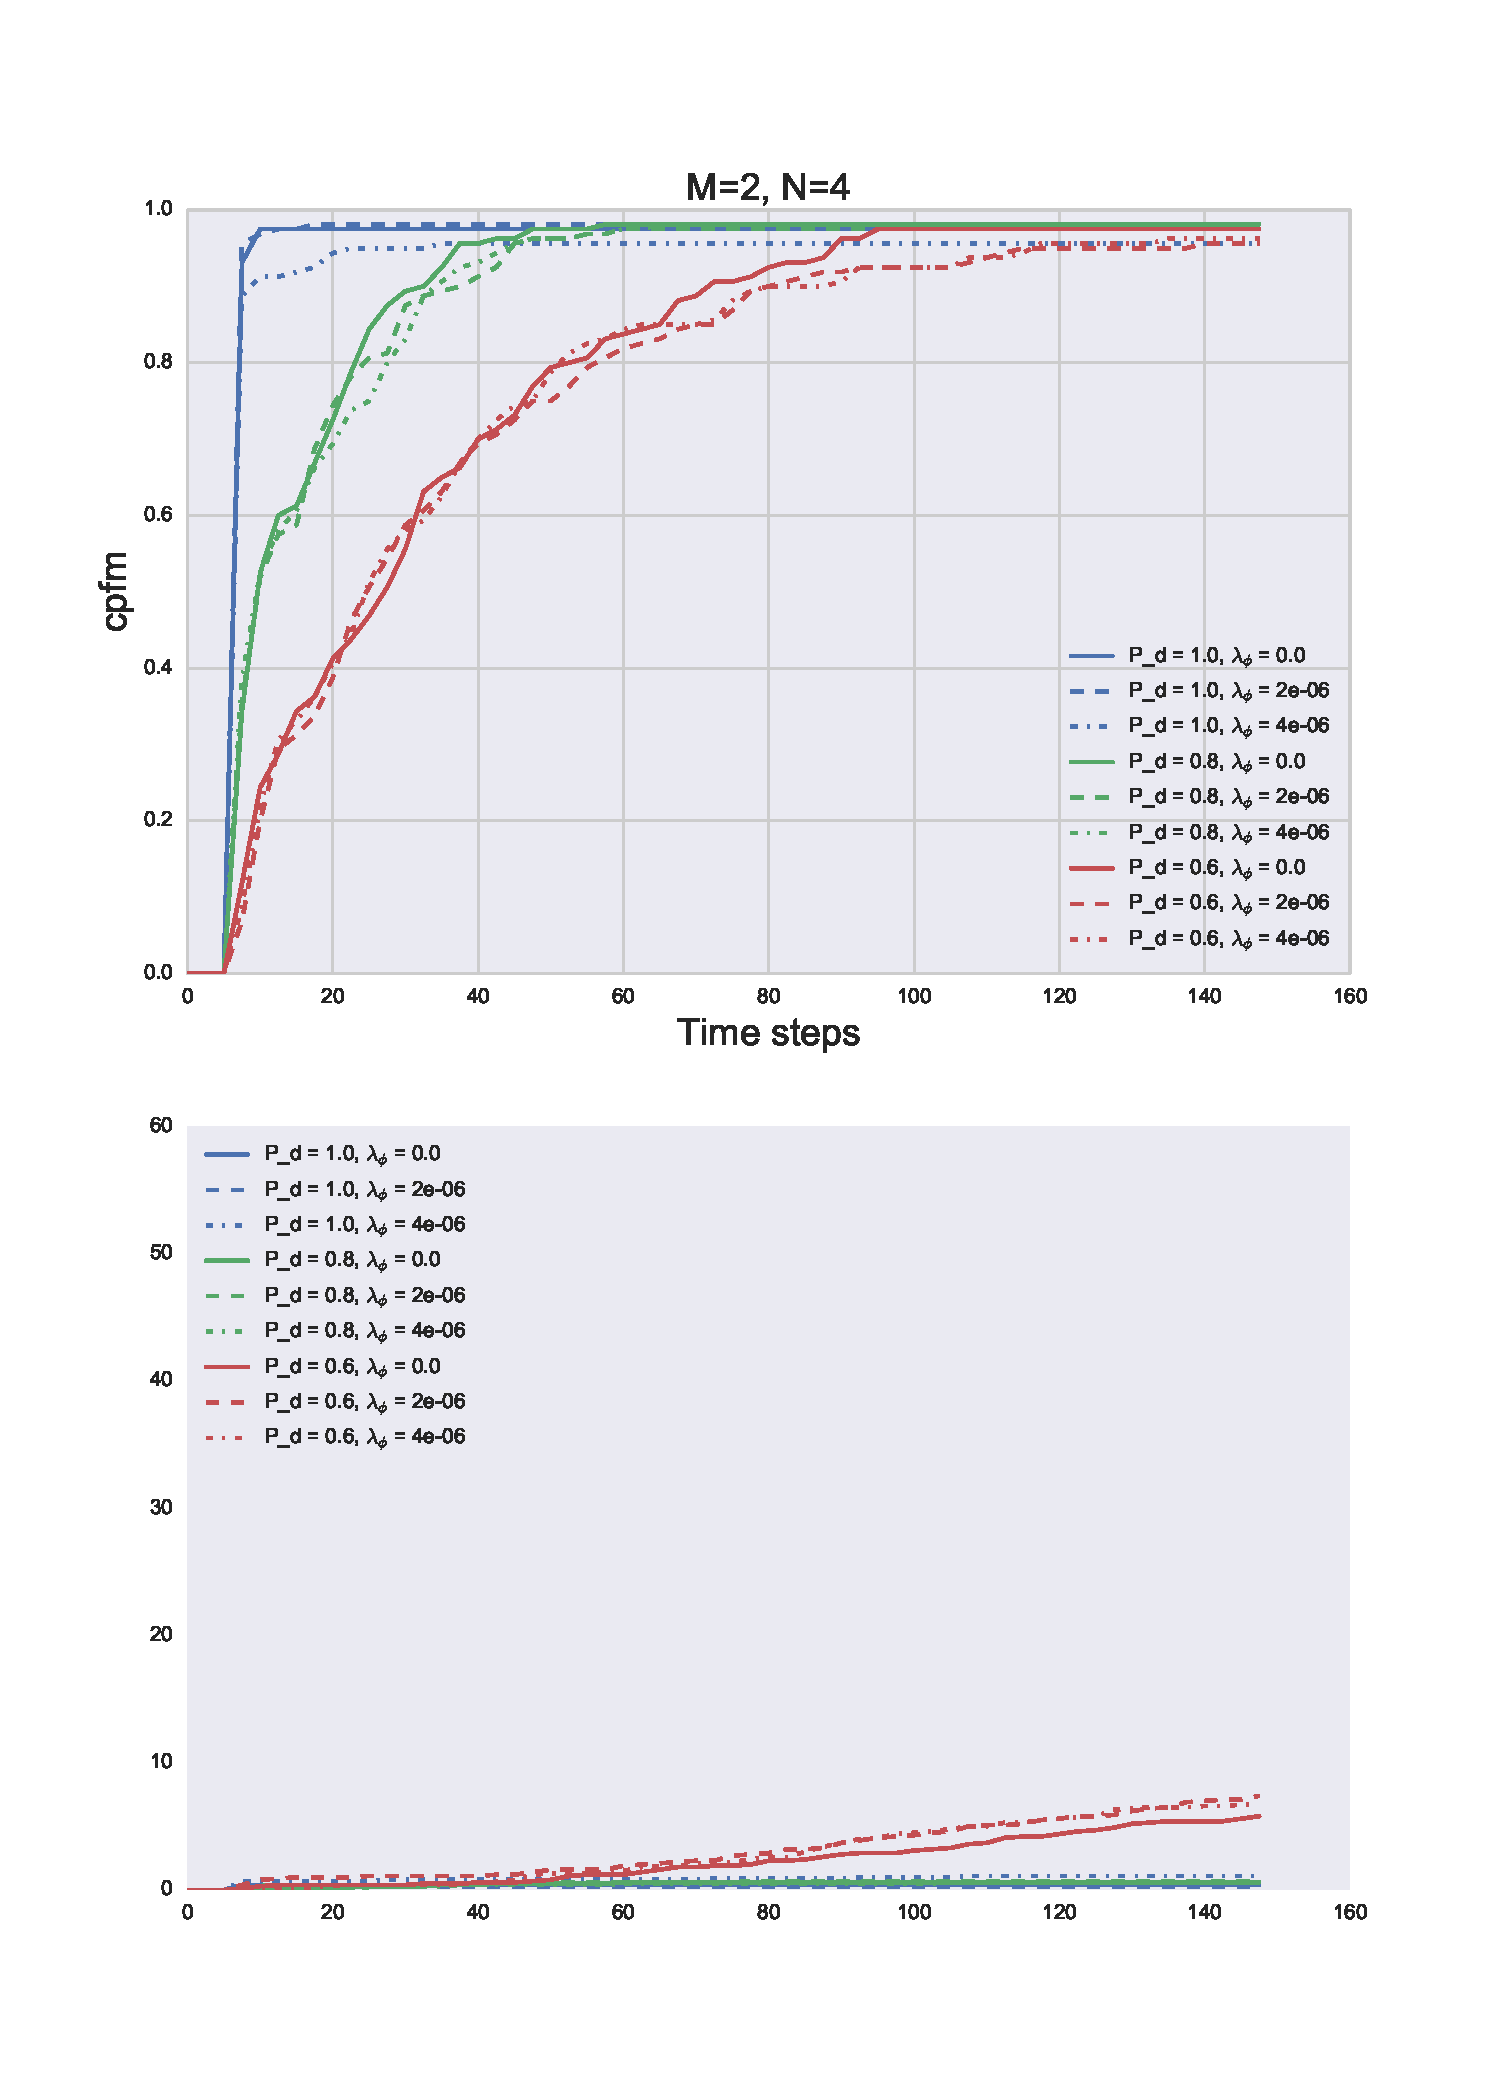
\includegraphics[height = .9\textheight]{Figures/plots/Scenario1_Init-Time(2-4).pdf}
\caption{Initialization time (2/4)}\label{fig:init_time_2-4}
\end{figure}

\begin{figure}
\centering
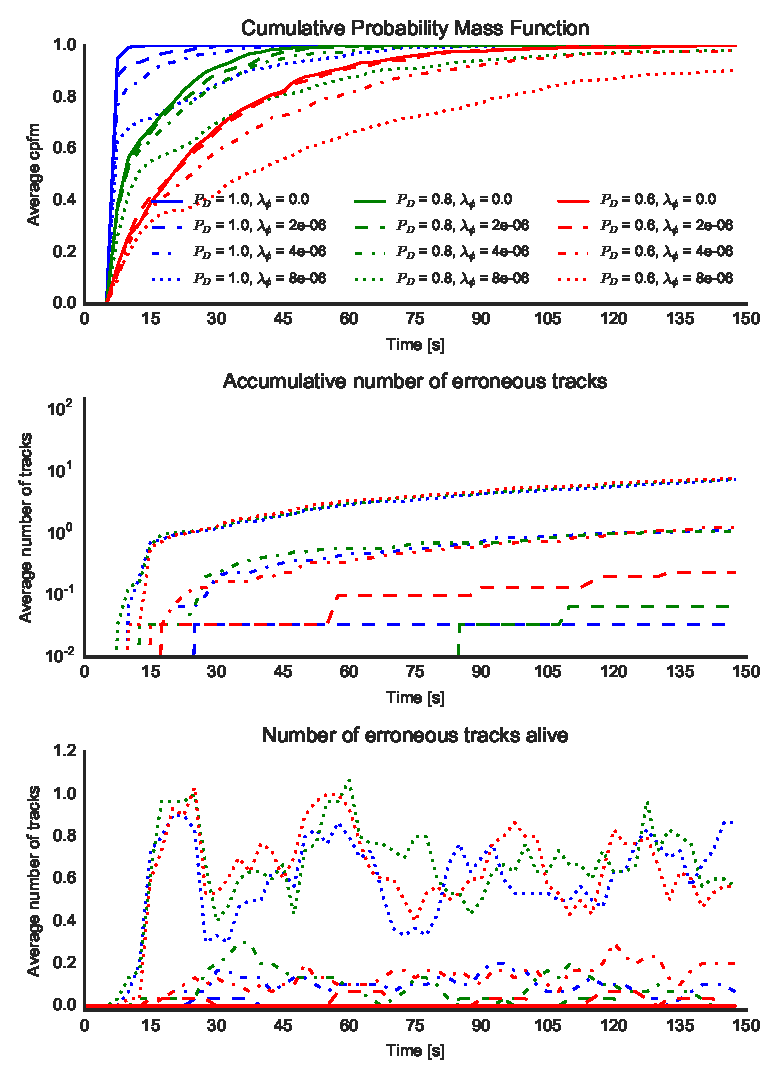
\includegraphics[height = .9\textheight]{Figures/plots/Scenario1_Init-Time(2-5).pdf}
\caption{Initialization time (2/5)}\label{fig:init_time_2-5}
\end{figure}

\begin{figure}
\centering
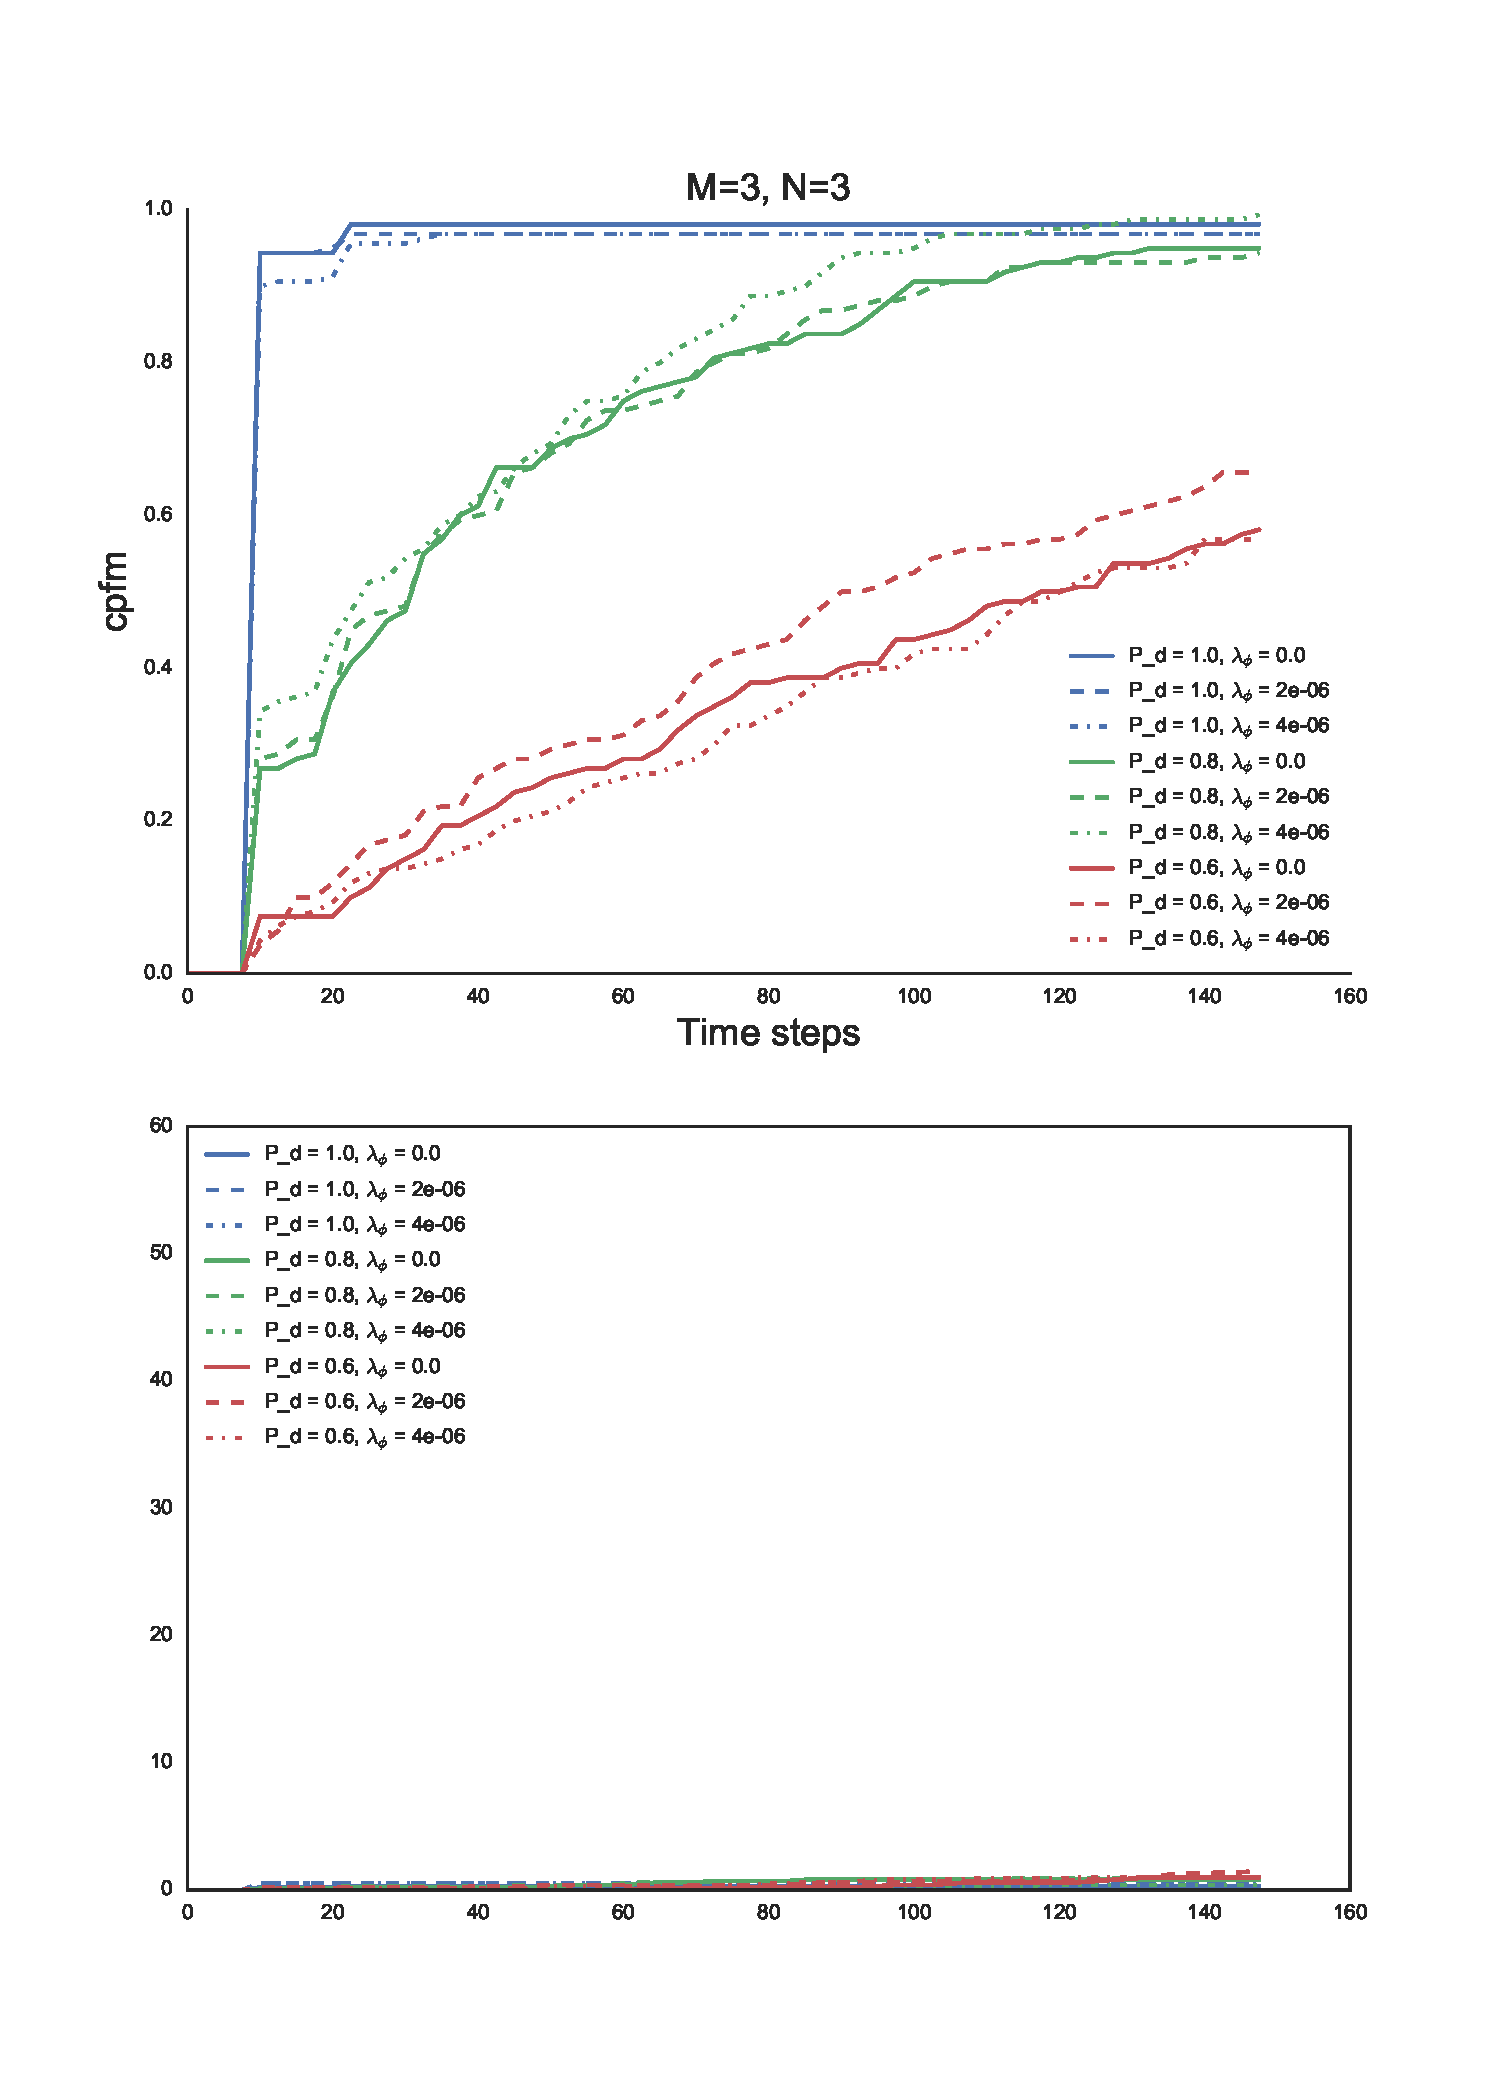
\includegraphics[height = .9\textheight]{Figures/plots/Scenario1_Init-Time(3-3).pdf}
\caption{Initialization time (3/3)}\label{fig:init_time_3-3}
\end{figure}

\begin{figure}
\centering
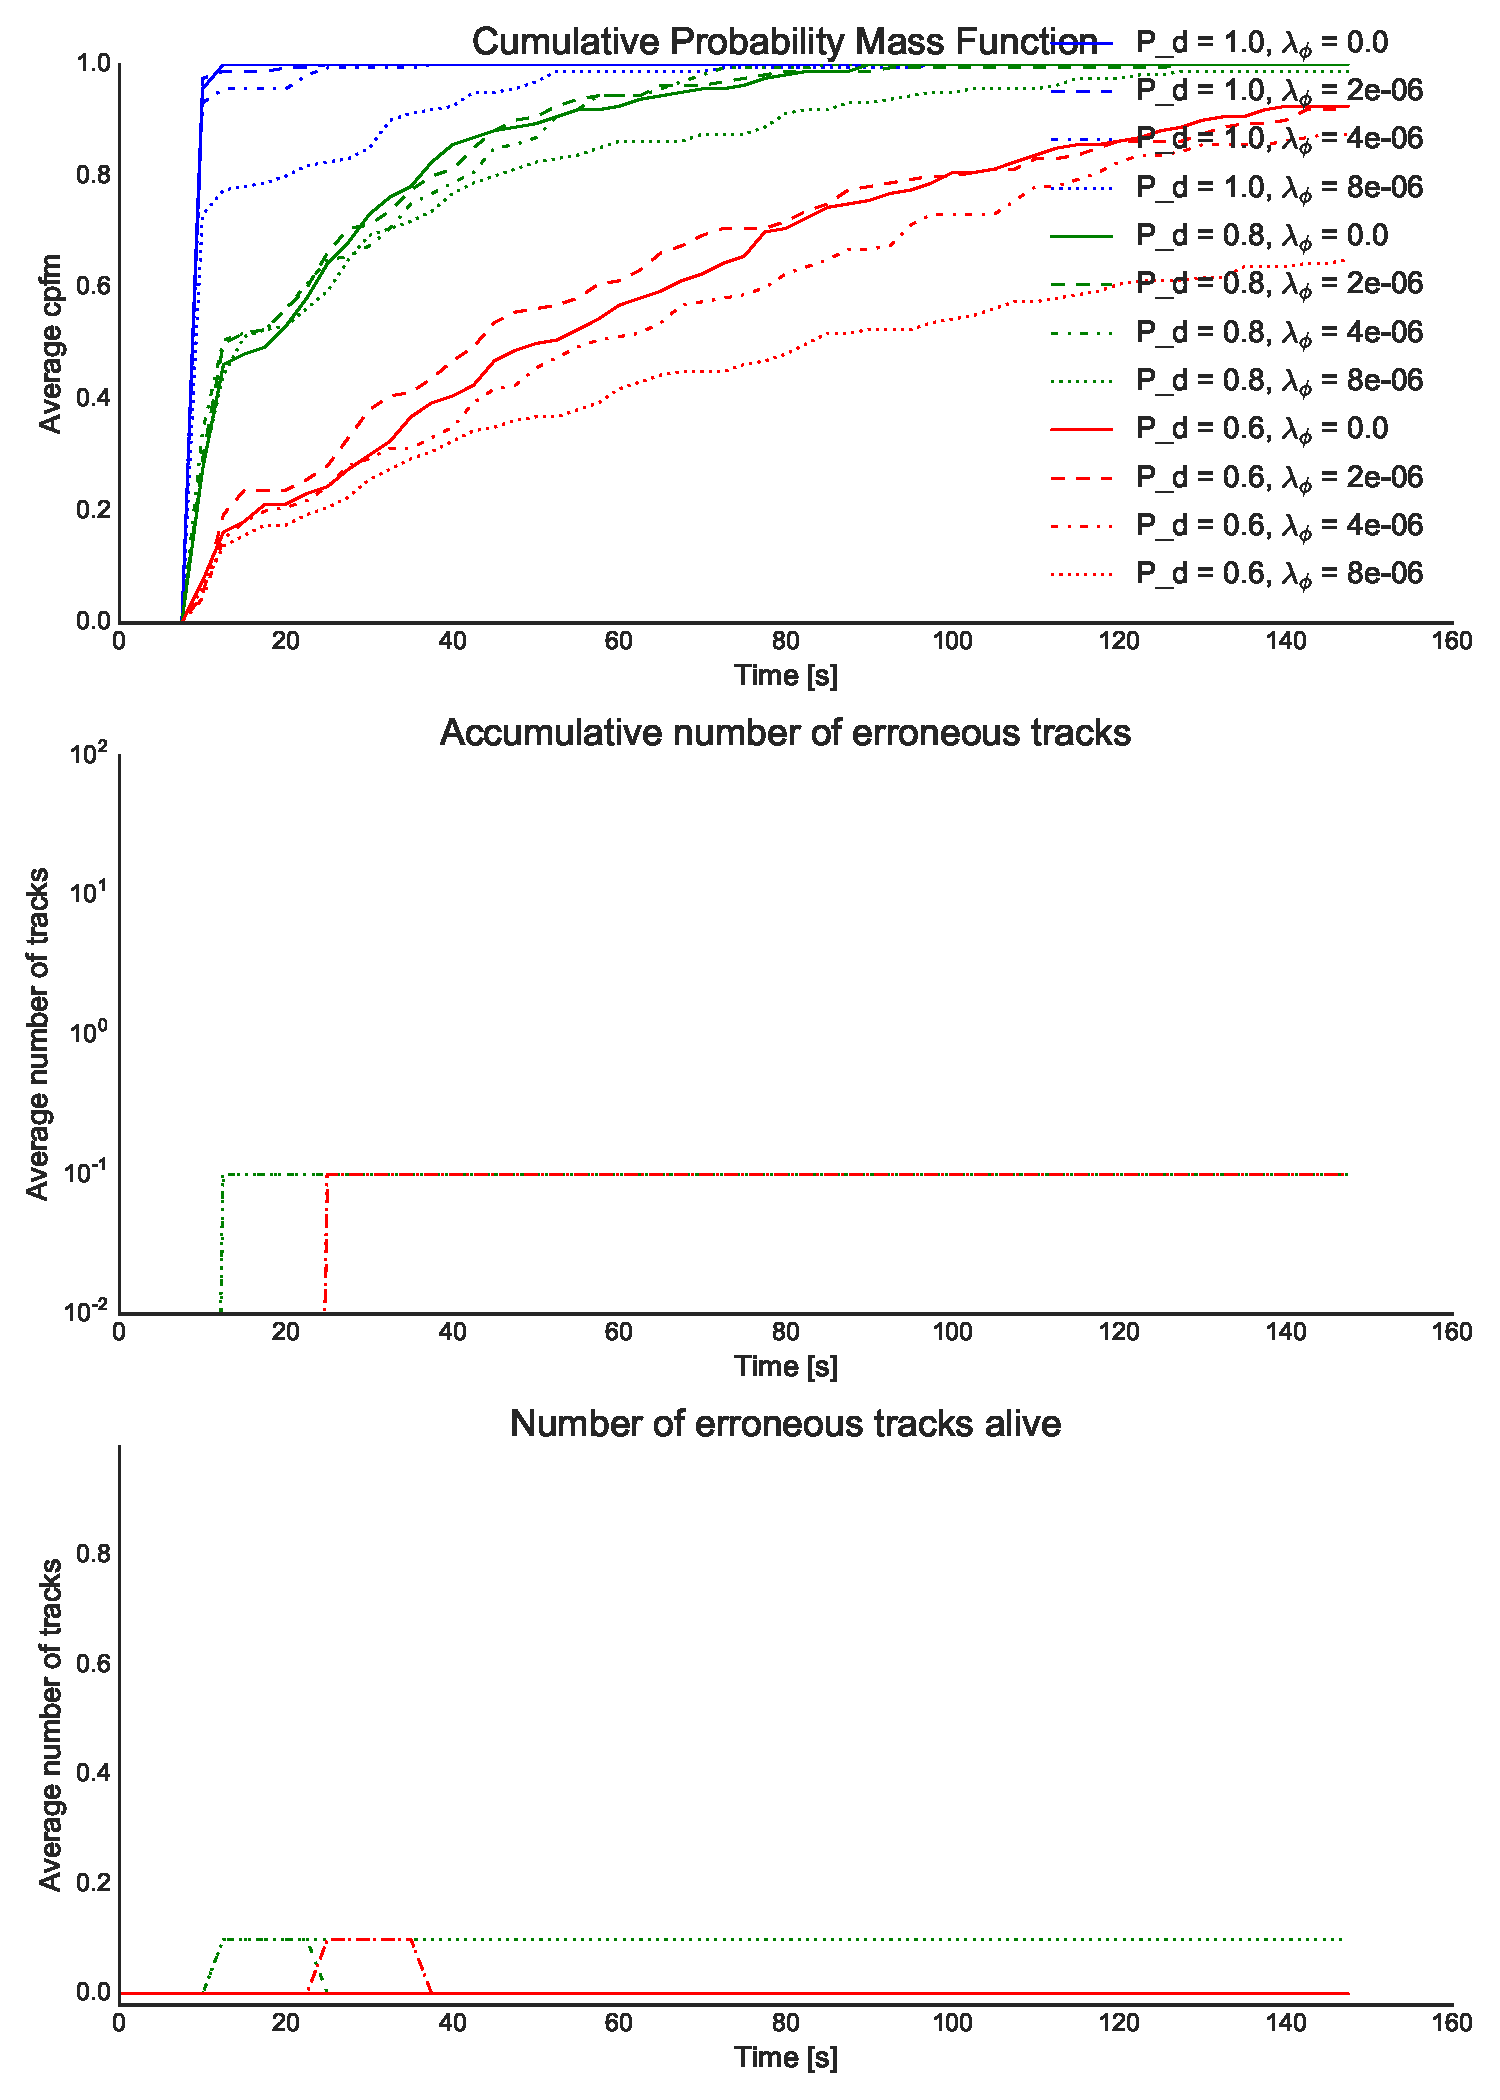
\includegraphics[height = .9\textheight]{Figures/plots/Scenario1_Init-Time(3-4).pdf}
\caption{Initialization time (3/4)}\label{fig:init_time_3-4}
\end{figure}

\begin{figure}
\centering
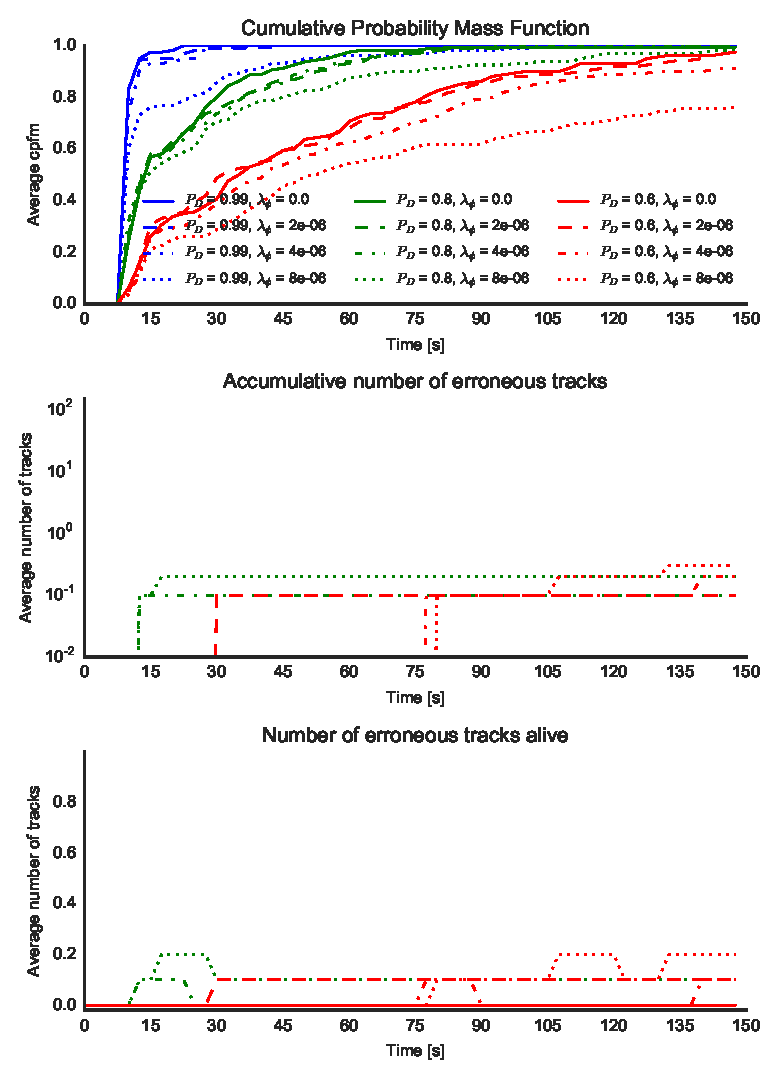
\includegraphics[height = .9\textheight]{Figures/plots/Scenario1_Init-Time(3-5).pdf}
\caption{Initialization time (3/5)}\label{fig:init_time_3-5}
\end{figure}

\begin{figure}
\centering
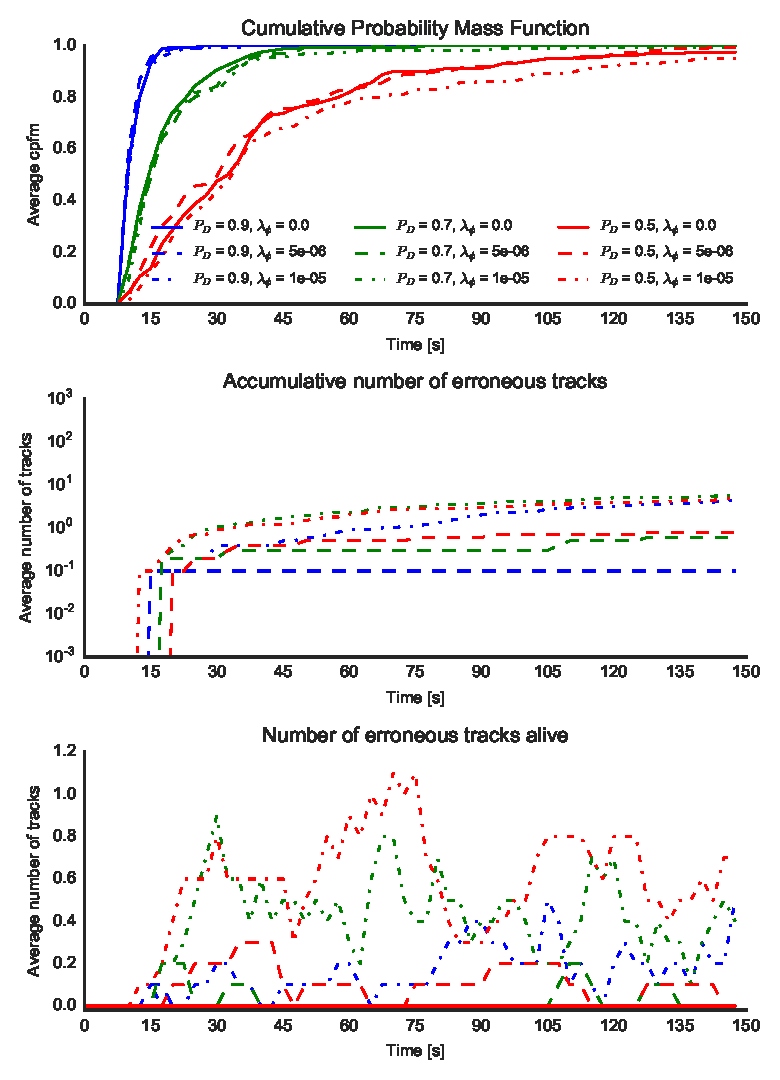
\includegraphics[height = .9\textheight]{Figures/plots/Scenario1_Init-Time(3-6).pdf}
\caption{Initialization time (3/6)}\label{fig:init_time_3-6}
\end{figure}
	%!TEX root = ../TTK4900-MHT.tex

\chapter{Track loss plot}
{
\setlength{\intextsep}{0mm}
\begin{figure}[H]
\centering
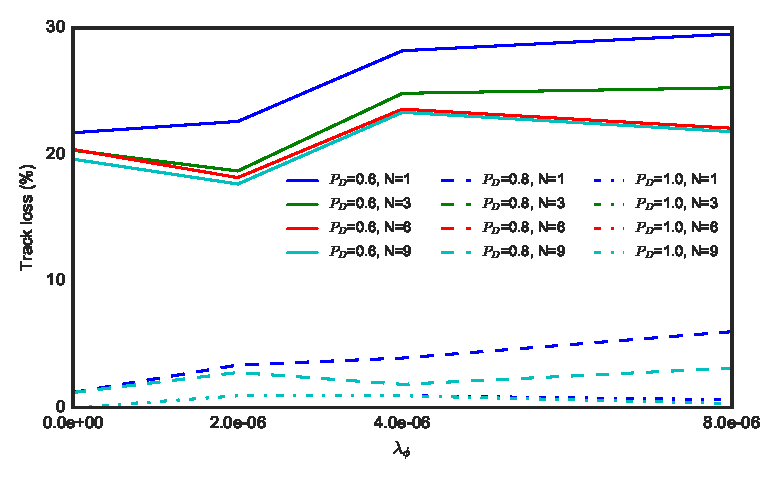
\includegraphics[height = .45\textheight]{Figures/plots/Scenario0_Tracking-TrackLoss.pdf}
\caption{Scenario 0 --- Track loss}\label{fig:scenario0_track_loss}
\end{figure}

\begin{figure}
\centering
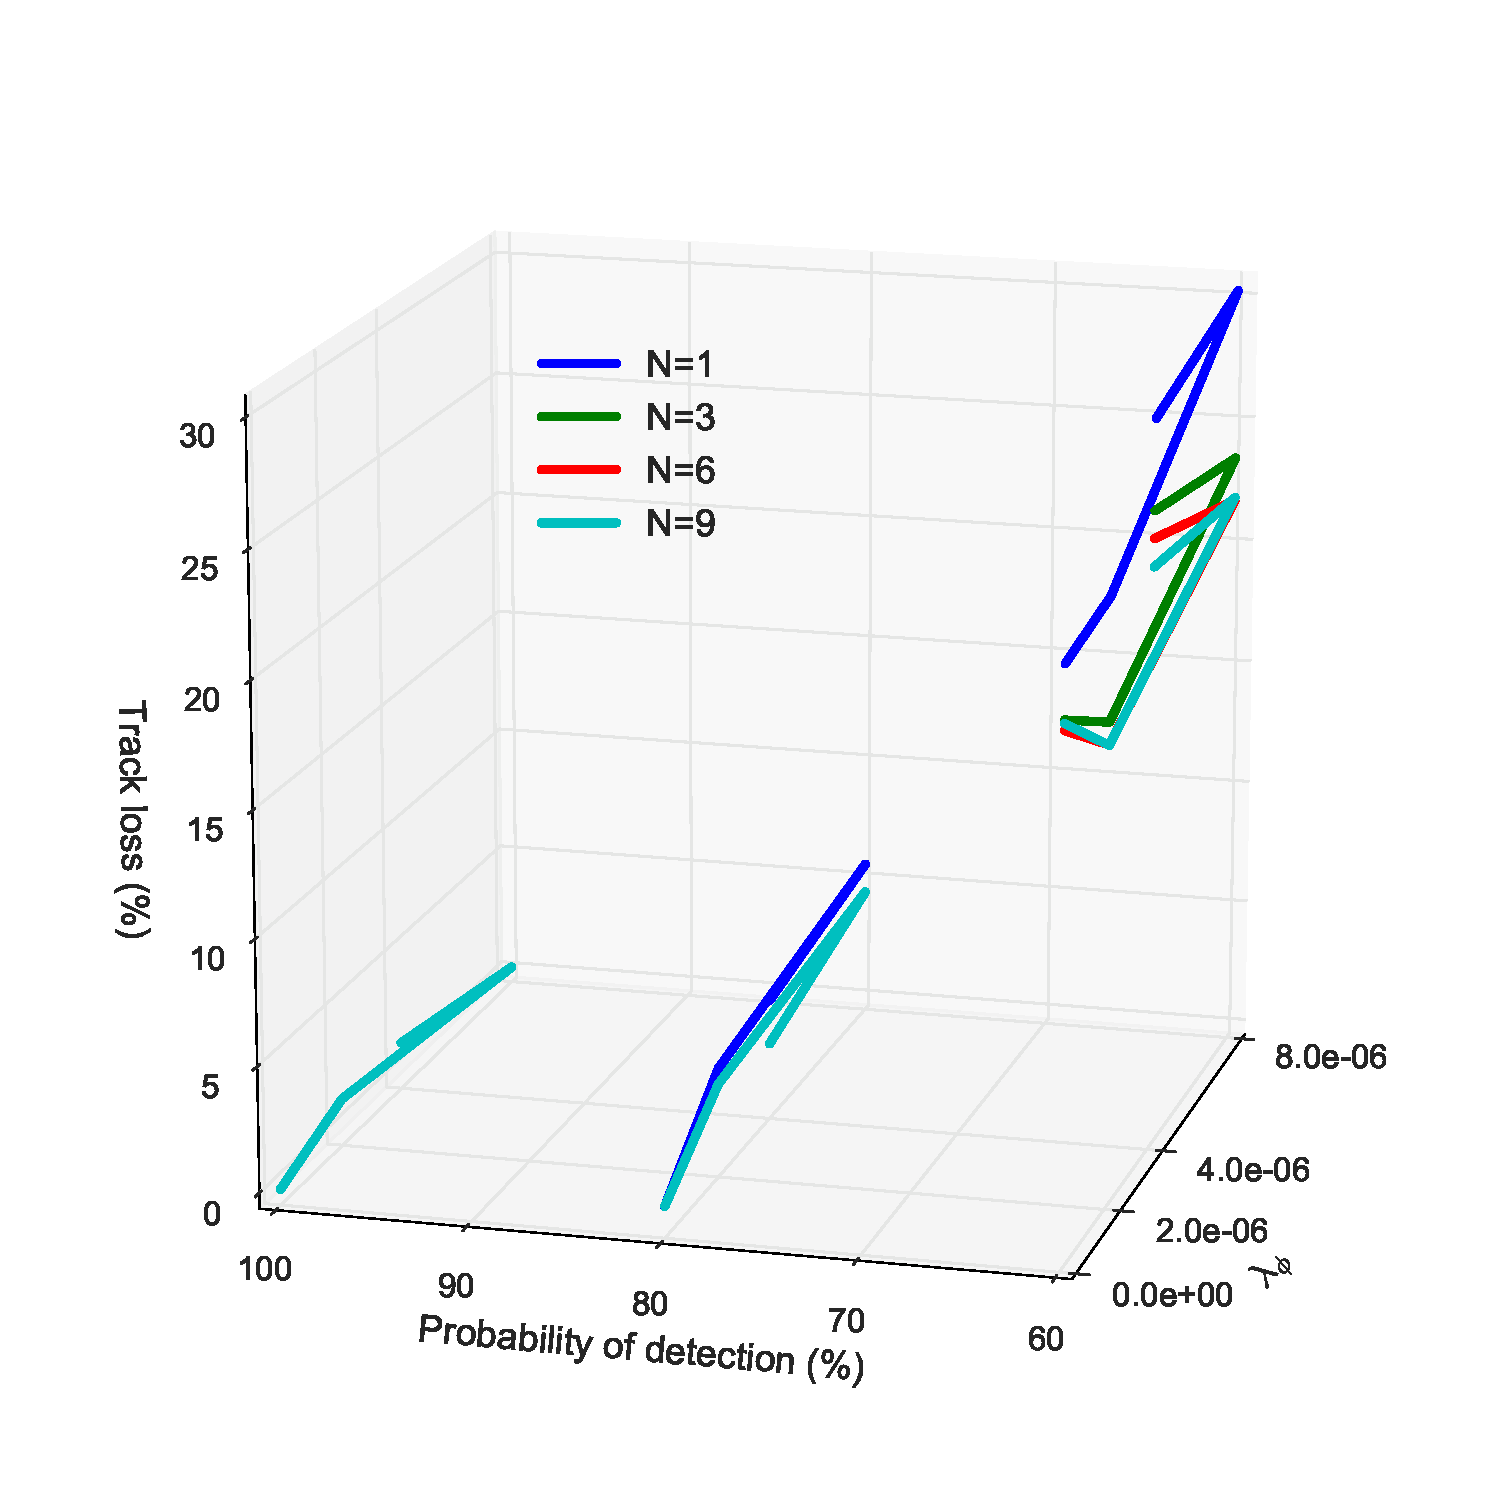
\includegraphics[height = .45\textheight]{Figures/plots/Scenario1_Tracking-TrackLoss.pdf}
\caption{Scenario 1 --- Track loss}\label{fig:scenario1_track_loss}

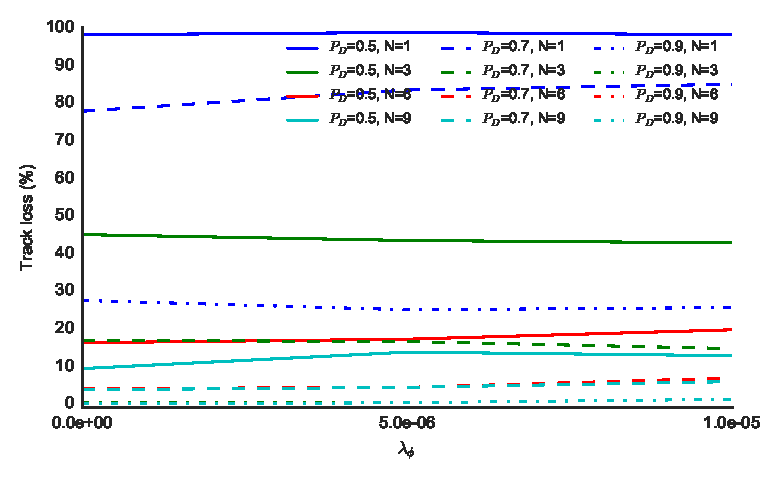
\includegraphics[height = .45\textheight]{Figures/plots/Scenario2_Tracking-TrackLoss.pdf}
\caption{Scenario 2 --- Track loss}\label{fig:scenario2_track_loss}
\end{figure}

\begin{figure}
\centering
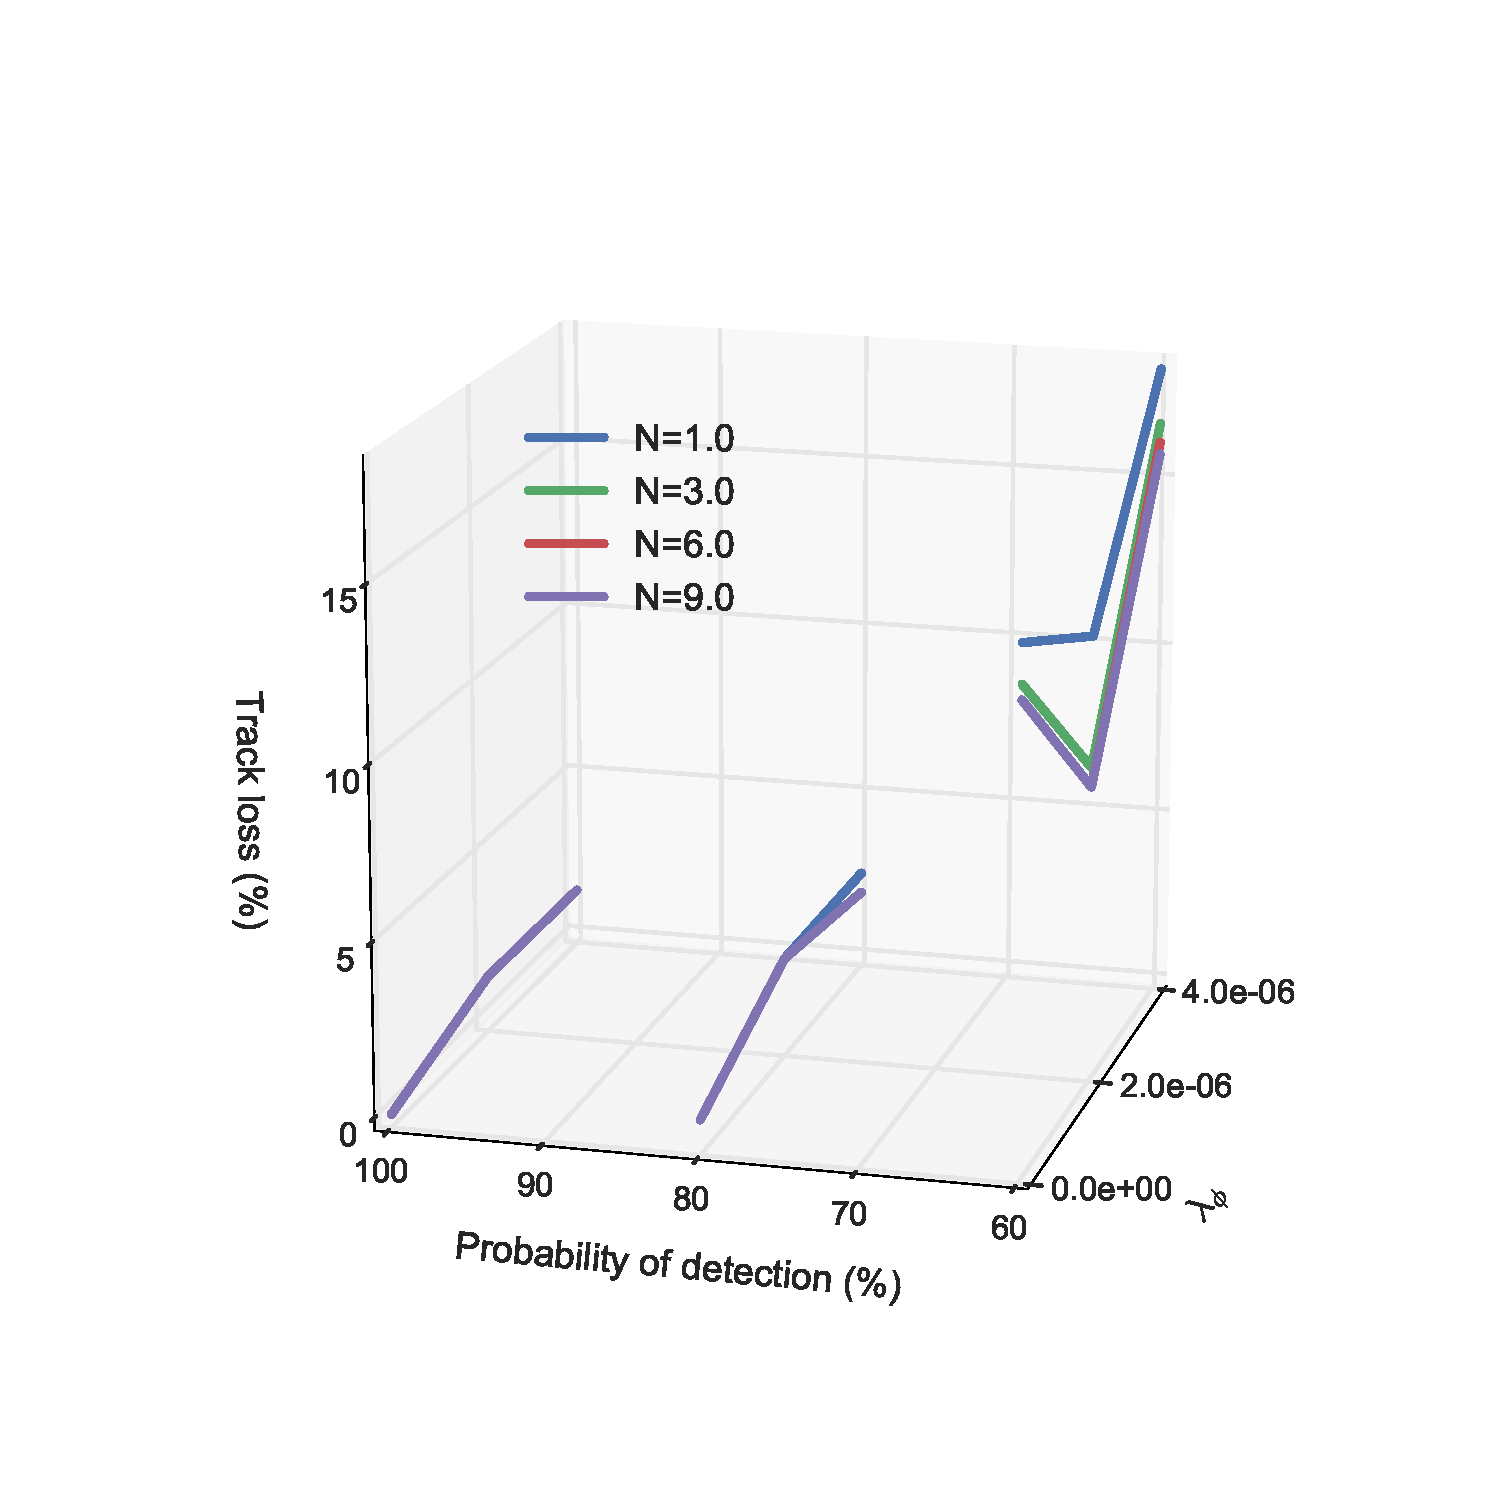
\includegraphics[height = .45\textheight]{Figures/plots/Scenario3_Tracking-TrackLoss.pdf}
\caption{Scenario 3 --- Track loss}\label{fig:scenario3_track_loss}

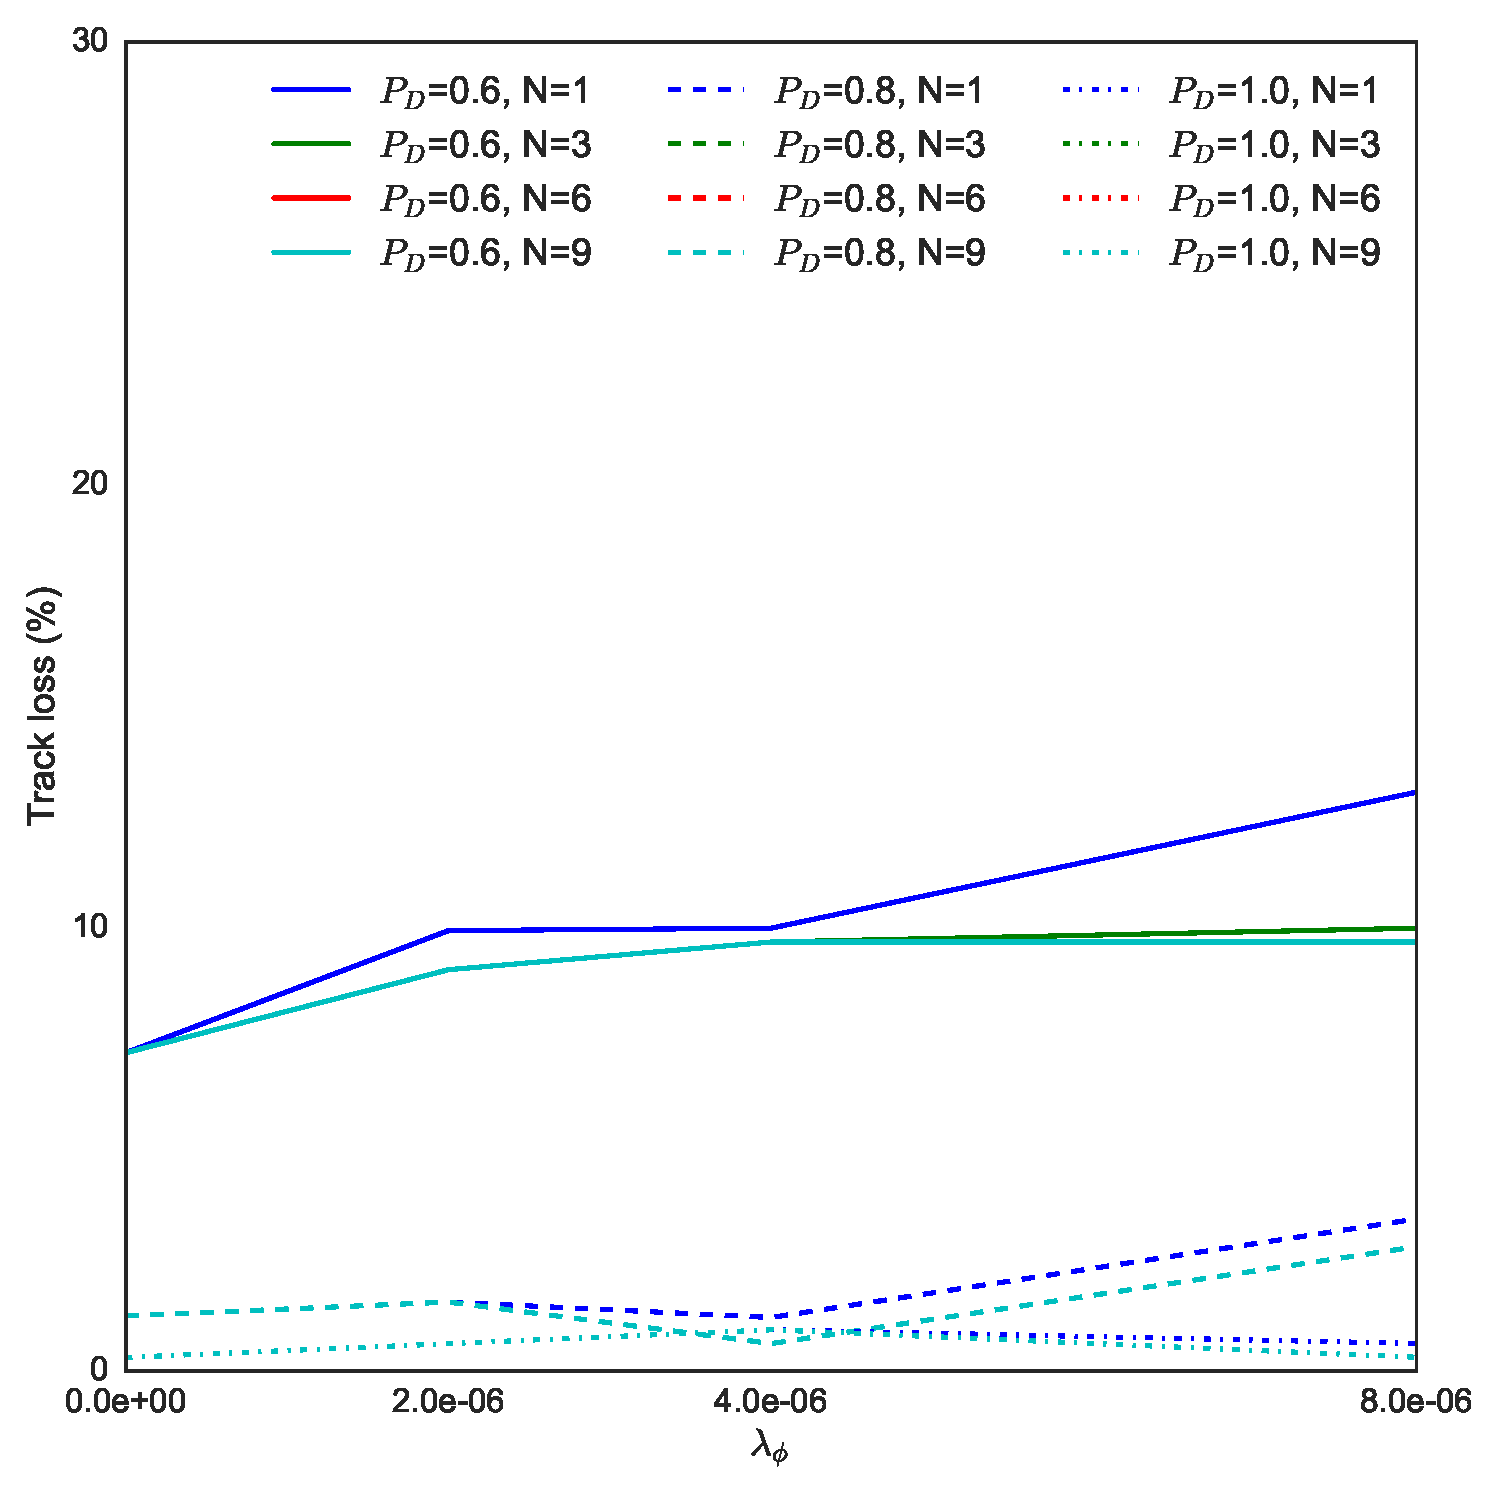
\includegraphics[height = .45\textheight]{Figures/plots/Scenario4_Tracking-TrackLoss.pdf}
\caption{Scenario 4 --- Track loss}\label{fig:scenario4_track_loss}
\end{figure}

}
	%!TEX root = ../TTK4900-MHT.tex

\chapter{Tracking percentage plot}
{
\setlength{\intextsep}{0mm}
\begin{figure}[H]
\centering
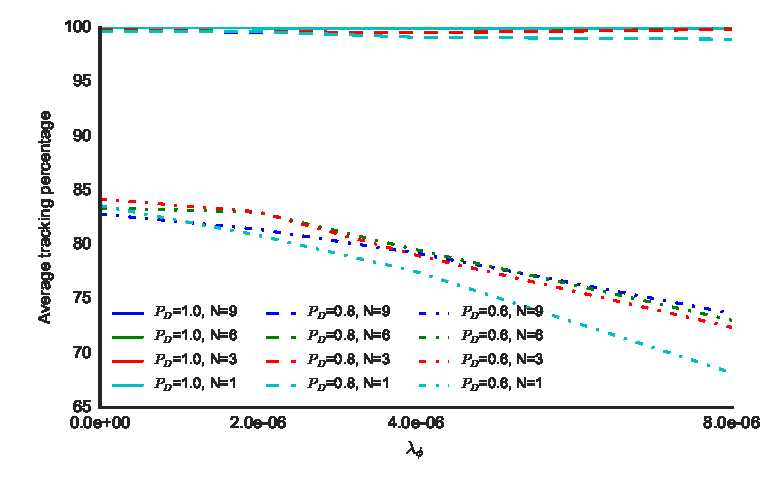
\includegraphics[height = .46\textheight]{Figures/plots/Scenario0_Tracking-TrackingPercentage.pdf}
\caption{Scenario 0 --- Tracking percentage}\label{fig:scenario0_tracking_percentage}
\end{figure}

\begin{figure}
\centering
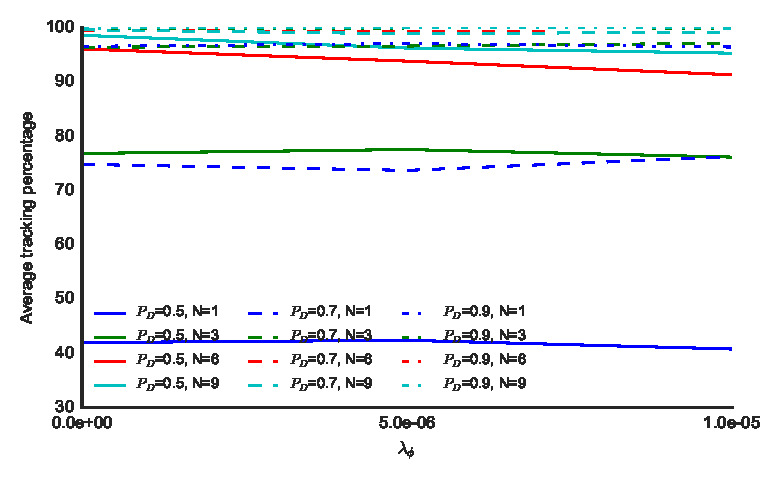
\includegraphics[height = .46\textheight]{Figures/plots/Scenario1_Tracking-TrackingPercentage.pdf}
\caption{Scenario 1 --- Tracking percentage}\label{fig:scenario1_tracking_percentage}

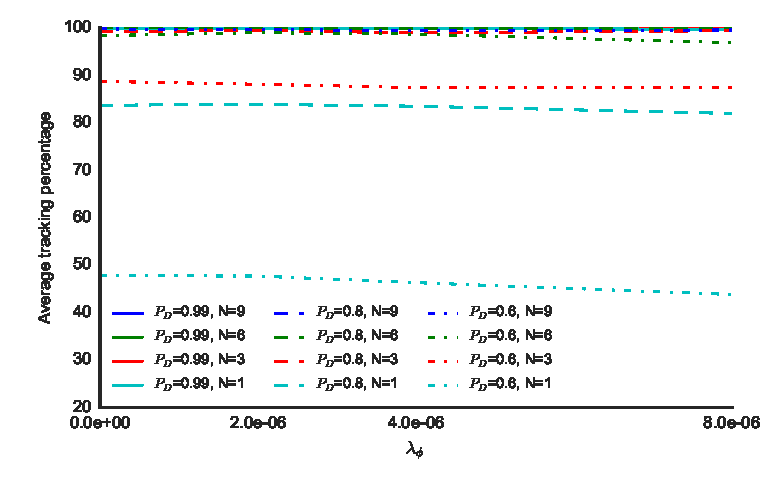
\includegraphics[height = .46\textheight]{Figures/plots/Scenario2_Tracking-TrackingPercentage.pdf}
\caption{Scenario 2 --- Tracking percentage}\label{fig:scenario2_tracking_percentage}
\end{figure}

\begin{figure}
\centering
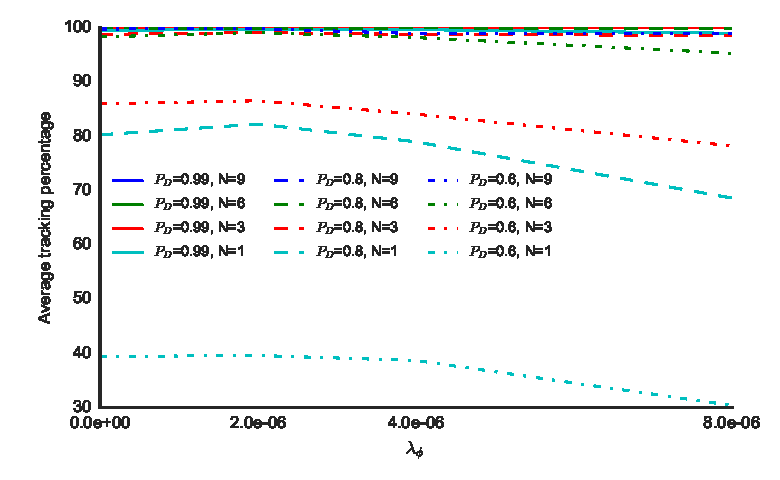
\includegraphics[height = .46\textheight]{Figures/plots/Scenario3_Tracking-TrackingPercentage.pdf}
\caption{Scenario 3 --- Tracking percentage}\label{fig:scenario3_tracking_percentage}

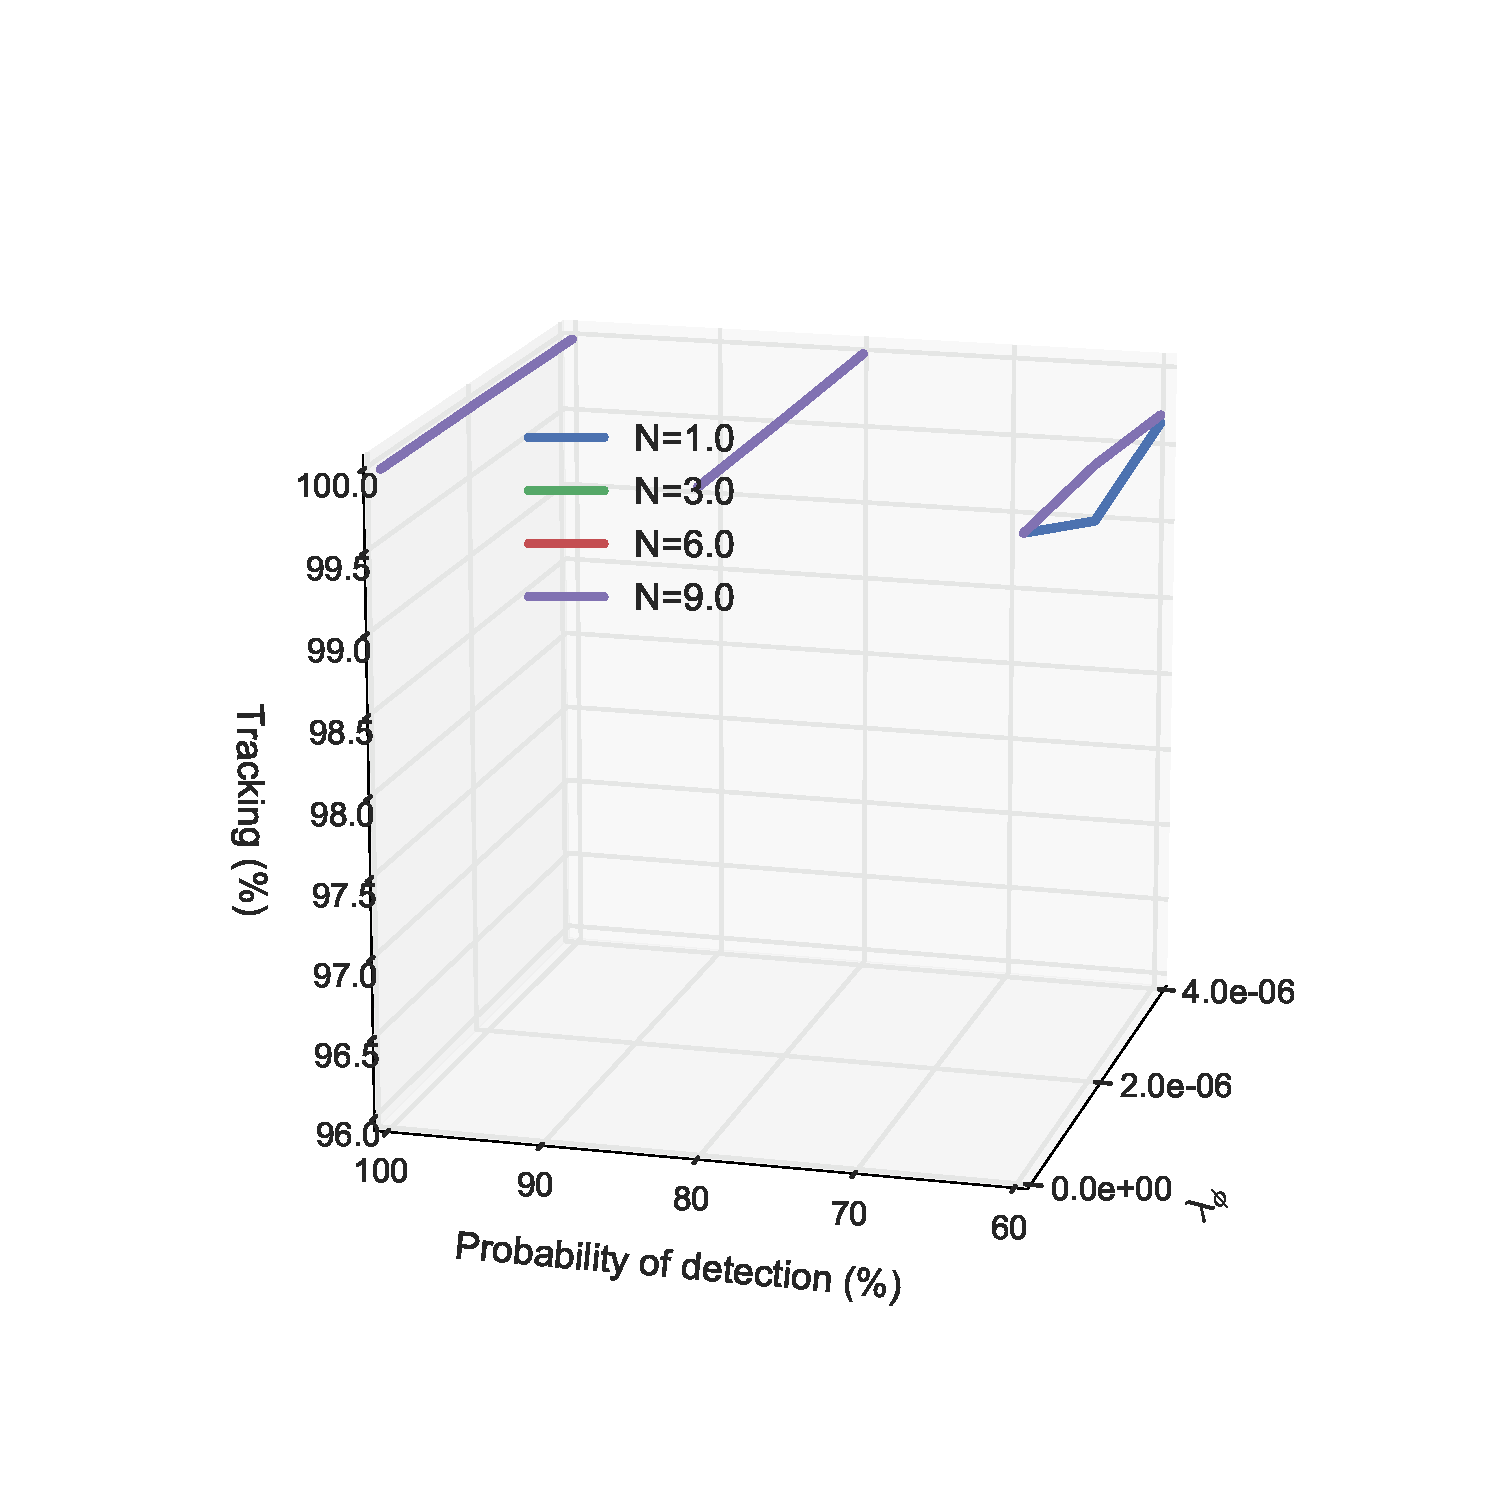
\includegraphics[height = .46\textheight]{Figures/plots/Scenario4_Tracking-TrackingPercentage.pdf}
\caption{Scenario 4 --- Tracking percentage}\label{fig:scenario4_tracking_percentage}
\end{figure}

}
\end{appendices} \clearpage
	\printbibliography{}
\end{document}